
% Default to the notebook output style

    


% Inherit from the specified cell style.




    
\documentclass[11pt]{article}

    
    
    \usepackage[T1]{fontenc}
    % Nicer default font (+ math font) than Computer Modern for most use cases
    \usepackage{mathpazo}

    % Basic figure setup, for now with no caption control since it's done
    % automatically by Pandoc (which extracts ![](path) syntax from Markdown).
    \usepackage{graphicx}
    % We will generate all images so they have a width \maxwidth. This means
    % that they will get their normal width if they fit onto the page, but
    % are scaled down if they would overflow the margins.
    \makeatletter
    \def\maxwidth{\ifdim\Gin@nat@width>\linewidth\linewidth
    \else\Gin@nat@width\fi}
    \makeatother
    \let\Oldincludegraphics\includegraphics
    % Set max figure width to be 80% of text width, for now hardcoded.
    \renewcommand{\includegraphics}[1]{\Oldincludegraphics[width=.8\maxwidth]{#1}}
    % Ensure that by default, figures have no caption (until we provide a
    % proper Figure object with a Caption API and a way to capture that
    % in the conversion process - todo).
    \usepackage{caption}
    \DeclareCaptionLabelFormat{nolabel}{}
    \captionsetup{labelformat=nolabel}

    \usepackage{adjustbox} % Used to constrain images to a maximum size 
    \usepackage{xcolor} % Allow colors to be defined
    \usepackage{enumerate} % Needed for markdown enumerations to work
    \usepackage{geometry} % Used to adjust the document margins
    \usepackage{amsmath} % Equations
    \usepackage{amssymb} % Equations
    \usepackage{textcomp} % defines textquotesingle
    % Hack from http://tex.stackexchange.com/a/47451/13684:
    \AtBeginDocument{%
        \def\PYZsq{\textquotesingle}% Upright quotes in Pygmentized code
    }
    \usepackage{upquote} % Upright quotes for verbatim code
    \usepackage{eurosym} % defines \euro
    \usepackage[mathletters]{ucs} % Extended unicode (utf-8) support
    \usepackage[utf8x]{inputenc} % Allow utf-8 characters in the tex document
    \usepackage{fancyvrb} % verbatim replacement that allows latex
    \usepackage{grffile} % extends the file name processing of package graphics 
                         % to support a larger range 
    % The hyperref package gives us a pdf with properly built
    % internal navigation ('pdf bookmarks' for the table of contents,
    % internal cross-reference links, web links for URLs, etc.)
    \usepackage{hyperref}
    \usepackage{longtable} % longtable support required by pandoc >1.10
    \usepackage{booktabs}  % table support for pandoc > 1.12.2
    \usepackage[inline]{enumitem} % IRkernel/repr support (it uses the enumerate* environment)
    \usepackage[normalem]{ulem} % ulem is needed to support strikethroughs (\sout)
                                % normalem makes italics be italics, not underlines
    

    
    
    % Colors for the hyperref package
    \definecolor{urlcolor}{rgb}{0,.145,.698}
    \definecolor{linkcolor}{rgb}{.71,0.21,0.01}
    \definecolor{citecolor}{rgb}{.12,.54,.11}

    % ANSI colors
    \definecolor{ansi-black}{HTML}{3E424D}
    \definecolor{ansi-black-intense}{HTML}{282C36}
    \definecolor{ansi-red}{HTML}{E75C58}
    \definecolor{ansi-red-intense}{HTML}{B22B31}
    \definecolor{ansi-green}{HTML}{00A250}
    \definecolor{ansi-green-intense}{HTML}{007427}
    \definecolor{ansi-yellow}{HTML}{DDB62B}
    \definecolor{ansi-yellow-intense}{HTML}{B27D12}
    \definecolor{ansi-blue}{HTML}{208FFB}
    \definecolor{ansi-blue-intense}{HTML}{0065CA}
    \definecolor{ansi-magenta}{HTML}{D160C4}
    \definecolor{ansi-magenta-intense}{HTML}{A03196}
    \definecolor{ansi-cyan}{HTML}{60C6C8}
    \definecolor{ansi-cyan-intense}{HTML}{258F8F}
    \definecolor{ansi-white}{HTML}{C5C1B4}
    \definecolor{ansi-white-intense}{HTML}{A1A6B2}

    % commands and environments needed by pandoc snippets
    % extracted from the output of `pandoc -s`
    \providecommand{\tightlist}{%
      \setlength{\itemsep}{0pt}\setlength{\parskip}{0pt}}
    \DefineVerbatimEnvironment{Highlighting}{Verbatim}{commandchars=\\\{\}}
    % Add ',fontsize=\small' for more characters per line
    \newenvironment{Shaded}{}{}
    \newcommand{\KeywordTok}[1]{\textcolor[rgb]{0.00,0.44,0.13}{\textbf{{#1}}}}
    \newcommand{\DataTypeTok}[1]{\textcolor[rgb]{0.56,0.13,0.00}{{#1}}}
    \newcommand{\DecValTok}[1]{\textcolor[rgb]{0.25,0.63,0.44}{{#1}}}
    \newcommand{\BaseNTok}[1]{\textcolor[rgb]{0.25,0.63,0.44}{{#1}}}
    \newcommand{\FloatTok}[1]{\textcolor[rgb]{0.25,0.63,0.44}{{#1}}}
    \newcommand{\CharTok}[1]{\textcolor[rgb]{0.25,0.44,0.63}{{#1}}}
    \newcommand{\StringTok}[1]{\textcolor[rgb]{0.25,0.44,0.63}{{#1}}}
    \newcommand{\CommentTok}[1]{\textcolor[rgb]{0.38,0.63,0.69}{\textit{{#1}}}}
    \newcommand{\OtherTok}[1]{\textcolor[rgb]{0.00,0.44,0.13}{{#1}}}
    \newcommand{\AlertTok}[1]{\textcolor[rgb]{1.00,0.00,0.00}{\textbf{{#1}}}}
    \newcommand{\FunctionTok}[1]{\textcolor[rgb]{0.02,0.16,0.49}{{#1}}}
    \newcommand{\RegionMarkerTok}[1]{{#1}}
    \newcommand{\ErrorTok}[1]{\textcolor[rgb]{1.00,0.00,0.00}{\textbf{{#1}}}}
    \newcommand{\NormalTok}[1]{{#1}}
    
    % Additional commands for more recent versions of Pandoc
    \newcommand{\ConstantTok}[1]{\textcolor[rgb]{0.53,0.00,0.00}{{#1}}}
    \newcommand{\SpecialCharTok}[1]{\textcolor[rgb]{0.25,0.44,0.63}{{#1}}}
    \newcommand{\VerbatimStringTok}[1]{\textcolor[rgb]{0.25,0.44,0.63}{{#1}}}
    \newcommand{\SpecialStringTok}[1]{\textcolor[rgb]{0.73,0.40,0.53}{{#1}}}
    \newcommand{\ImportTok}[1]{{#1}}
    \newcommand{\DocumentationTok}[1]{\textcolor[rgb]{0.73,0.13,0.13}{\textit{{#1}}}}
    \newcommand{\AnnotationTok}[1]{\textcolor[rgb]{0.38,0.63,0.69}{\textbf{\textit{{#1}}}}}
    \newcommand{\CommentVarTok}[1]{\textcolor[rgb]{0.38,0.63,0.69}{\textbf{\textit{{#1}}}}}
    \newcommand{\VariableTok}[1]{\textcolor[rgb]{0.10,0.09,0.49}{{#1}}}
    \newcommand{\ControlFlowTok}[1]{\textcolor[rgb]{0.00,0.44,0.13}{\textbf{{#1}}}}
    \newcommand{\OperatorTok}[1]{\textcolor[rgb]{0.40,0.40,0.40}{{#1}}}
    \newcommand{\BuiltInTok}[1]{{#1}}
    \newcommand{\ExtensionTok}[1]{{#1}}
    \newcommand{\PreprocessorTok}[1]{\textcolor[rgb]{0.74,0.48,0.00}{{#1}}}
    \newcommand{\AttributeTok}[1]{\textcolor[rgb]{0.49,0.56,0.16}{{#1}}}
    \newcommand{\InformationTok}[1]{\textcolor[rgb]{0.38,0.63,0.69}{\textbf{\textit{{#1}}}}}
    \newcommand{\WarningTok}[1]{\textcolor[rgb]{0.38,0.63,0.69}{\textbf{\textit{{#1}}}}}
    
    
    % Define a nice break command that doesn't care if a line doesn't already
    % exist.
    \def\br{\hspace*{\fill} \\* }
    % Math Jax compatability definitions
    \def\gt{>}
    \def\lt{<}
    % Document parameters
    \title{HomeWork4\_M\_Kahack}
    
    
    

    % Pygments definitions
    
\makeatletter
\def\PY@reset{\let\PY@it=\relax \let\PY@bf=\relax%
    \let\PY@ul=\relax \let\PY@tc=\relax%
    \let\PY@bc=\relax \let\PY@ff=\relax}
\def\PY@tok#1{\csname PY@tok@#1\endcsname}
\def\PY@toks#1+{\ifx\relax#1\empty\else%
    \PY@tok{#1}\expandafter\PY@toks\fi}
\def\PY@do#1{\PY@bc{\PY@tc{\PY@ul{%
    \PY@it{\PY@bf{\PY@ff{#1}}}}}}}
\def\PY#1#2{\PY@reset\PY@toks#1+\relax+\PY@do{#2}}

\expandafter\def\csname PY@tok@w\endcsname{\def\PY@tc##1{\textcolor[rgb]{0.73,0.73,0.73}{##1}}}
\expandafter\def\csname PY@tok@c\endcsname{\let\PY@it=\textit\def\PY@tc##1{\textcolor[rgb]{0.25,0.50,0.50}{##1}}}
\expandafter\def\csname PY@tok@cp\endcsname{\def\PY@tc##1{\textcolor[rgb]{0.74,0.48,0.00}{##1}}}
\expandafter\def\csname PY@tok@k\endcsname{\let\PY@bf=\textbf\def\PY@tc##1{\textcolor[rgb]{0.00,0.50,0.00}{##1}}}
\expandafter\def\csname PY@tok@kp\endcsname{\def\PY@tc##1{\textcolor[rgb]{0.00,0.50,0.00}{##1}}}
\expandafter\def\csname PY@tok@kt\endcsname{\def\PY@tc##1{\textcolor[rgb]{0.69,0.00,0.25}{##1}}}
\expandafter\def\csname PY@tok@o\endcsname{\def\PY@tc##1{\textcolor[rgb]{0.40,0.40,0.40}{##1}}}
\expandafter\def\csname PY@tok@ow\endcsname{\let\PY@bf=\textbf\def\PY@tc##1{\textcolor[rgb]{0.67,0.13,1.00}{##1}}}
\expandafter\def\csname PY@tok@nb\endcsname{\def\PY@tc##1{\textcolor[rgb]{0.00,0.50,0.00}{##1}}}
\expandafter\def\csname PY@tok@nf\endcsname{\def\PY@tc##1{\textcolor[rgb]{0.00,0.00,1.00}{##1}}}
\expandafter\def\csname PY@tok@nc\endcsname{\let\PY@bf=\textbf\def\PY@tc##1{\textcolor[rgb]{0.00,0.00,1.00}{##1}}}
\expandafter\def\csname PY@tok@nn\endcsname{\let\PY@bf=\textbf\def\PY@tc##1{\textcolor[rgb]{0.00,0.00,1.00}{##1}}}
\expandafter\def\csname PY@tok@ne\endcsname{\let\PY@bf=\textbf\def\PY@tc##1{\textcolor[rgb]{0.82,0.25,0.23}{##1}}}
\expandafter\def\csname PY@tok@nv\endcsname{\def\PY@tc##1{\textcolor[rgb]{0.10,0.09,0.49}{##1}}}
\expandafter\def\csname PY@tok@no\endcsname{\def\PY@tc##1{\textcolor[rgb]{0.53,0.00,0.00}{##1}}}
\expandafter\def\csname PY@tok@nl\endcsname{\def\PY@tc##1{\textcolor[rgb]{0.63,0.63,0.00}{##1}}}
\expandafter\def\csname PY@tok@ni\endcsname{\let\PY@bf=\textbf\def\PY@tc##1{\textcolor[rgb]{0.60,0.60,0.60}{##1}}}
\expandafter\def\csname PY@tok@na\endcsname{\def\PY@tc##1{\textcolor[rgb]{0.49,0.56,0.16}{##1}}}
\expandafter\def\csname PY@tok@nt\endcsname{\let\PY@bf=\textbf\def\PY@tc##1{\textcolor[rgb]{0.00,0.50,0.00}{##1}}}
\expandafter\def\csname PY@tok@nd\endcsname{\def\PY@tc##1{\textcolor[rgb]{0.67,0.13,1.00}{##1}}}
\expandafter\def\csname PY@tok@s\endcsname{\def\PY@tc##1{\textcolor[rgb]{0.73,0.13,0.13}{##1}}}
\expandafter\def\csname PY@tok@sd\endcsname{\let\PY@it=\textit\def\PY@tc##1{\textcolor[rgb]{0.73,0.13,0.13}{##1}}}
\expandafter\def\csname PY@tok@si\endcsname{\let\PY@bf=\textbf\def\PY@tc##1{\textcolor[rgb]{0.73,0.40,0.53}{##1}}}
\expandafter\def\csname PY@tok@se\endcsname{\let\PY@bf=\textbf\def\PY@tc##1{\textcolor[rgb]{0.73,0.40,0.13}{##1}}}
\expandafter\def\csname PY@tok@sr\endcsname{\def\PY@tc##1{\textcolor[rgb]{0.73,0.40,0.53}{##1}}}
\expandafter\def\csname PY@tok@ss\endcsname{\def\PY@tc##1{\textcolor[rgb]{0.10,0.09,0.49}{##1}}}
\expandafter\def\csname PY@tok@sx\endcsname{\def\PY@tc##1{\textcolor[rgb]{0.00,0.50,0.00}{##1}}}
\expandafter\def\csname PY@tok@m\endcsname{\def\PY@tc##1{\textcolor[rgb]{0.40,0.40,0.40}{##1}}}
\expandafter\def\csname PY@tok@gh\endcsname{\let\PY@bf=\textbf\def\PY@tc##1{\textcolor[rgb]{0.00,0.00,0.50}{##1}}}
\expandafter\def\csname PY@tok@gu\endcsname{\let\PY@bf=\textbf\def\PY@tc##1{\textcolor[rgb]{0.50,0.00,0.50}{##1}}}
\expandafter\def\csname PY@tok@gd\endcsname{\def\PY@tc##1{\textcolor[rgb]{0.63,0.00,0.00}{##1}}}
\expandafter\def\csname PY@tok@gi\endcsname{\def\PY@tc##1{\textcolor[rgb]{0.00,0.63,0.00}{##1}}}
\expandafter\def\csname PY@tok@gr\endcsname{\def\PY@tc##1{\textcolor[rgb]{1.00,0.00,0.00}{##1}}}
\expandafter\def\csname PY@tok@ge\endcsname{\let\PY@it=\textit}
\expandafter\def\csname PY@tok@gs\endcsname{\let\PY@bf=\textbf}
\expandafter\def\csname PY@tok@gp\endcsname{\let\PY@bf=\textbf\def\PY@tc##1{\textcolor[rgb]{0.00,0.00,0.50}{##1}}}
\expandafter\def\csname PY@tok@go\endcsname{\def\PY@tc##1{\textcolor[rgb]{0.53,0.53,0.53}{##1}}}
\expandafter\def\csname PY@tok@gt\endcsname{\def\PY@tc##1{\textcolor[rgb]{0.00,0.27,0.87}{##1}}}
\expandafter\def\csname PY@tok@err\endcsname{\def\PY@bc##1{\setlength{\fboxsep}{0pt}\fcolorbox[rgb]{1.00,0.00,0.00}{1,1,1}{\strut ##1}}}
\expandafter\def\csname PY@tok@kc\endcsname{\let\PY@bf=\textbf\def\PY@tc##1{\textcolor[rgb]{0.00,0.50,0.00}{##1}}}
\expandafter\def\csname PY@tok@kd\endcsname{\let\PY@bf=\textbf\def\PY@tc##1{\textcolor[rgb]{0.00,0.50,0.00}{##1}}}
\expandafter\def\csname PY@tok@kn\endcsname{\let\PY@bf=\textbf\def\PY@tc##1{\textcolor[rgb]{0.00,0.50,0.00}{##1}}}
\expandafter\def\csname PY@tok@kr\endcsname{\let\PY@bf=\textbf\def\PY@tc##1{\textcolor[rgb]{0.00,0.50,0.00}{##1}}}
\expandafter\def\csname PY@tok@bp\endcsname{\def\PY@tc##1{\textcolor[rgb]{0.00,0.50,0.00}{##1}}}
\expandafter\def\csname PY@tok@fm\endcsname{\def\PY@tc##1{\textcolor[rgb]{0.00,0.00,1.00}{##1}}}
\expandafter\def\csname PY@tok@vc\endcsname{\def\PY@tc##1{\textcolor[rgb]{0.10,0.09,0.49}{##1}}}
\expandafter\def\csname PY@tok@vg\endcsname{\def\PY@tc##1{\textcolor[rgb]{0.10,0.09,0.49}{##1}}}
\expandafter\def\csname PY@tok@vi\endcsname{\def\PY@tc##1{\textcolor[rgb]{0.10,0.09,0.49}{##1}}}
\expandafter\def\csname PY@tok@vm\endcsname{\def\PY@tc##1{\textcolor[rgb]{0.10,0.09,0.49}{##1}}}
\expandafter\def\csname PY@tok@sa\endcsname{\def\PY@tc##1{\textcolor[rgb]{0.73,0.13,0.13}{##1}}}
\expandafter\def\csname PY@tok@sb\endcsname{\def\PY@tc##1{\textcolor[rgb]{0.73,0.13,0.13}{##1}}}
\expandafter\def\csname PY@tok@sc\endcsname{\def\PY@tc##1{\textcolor[rgb]{0.73,0.13,0.13}{##1}}}
\expandafter\def\csname PY@tok@dl\endcsname{\def\PY@tc##1{\textcolor[rgb]{0.73,0.13,0.13}{##1}}}
\expandafter\def\csname PY@tok@s2\endcsname{\def\PY@tc##1{\textcolor[rgb]{0.73,0.13,0.13}{##1}}}
\expandafter\def\csname PY@tok@sh\endcsname{\def\PY@tc##1{\textcolor[rgb]{0.73,0.13,0.13}{##1}}}
\expandafter\def\csname PY@tok@s1\endcsname{\def\PY@tc##1{\textcolor[rgb]{0.73,0.13,0.13}{##1}}}
\expandafter\def\csname PY@tok@mb\endcsname{\def\PY@tc##1{\textcolor[rgb]{0.40,0.40,0.40}{##1}}}
\expandafter\def\csname PY@tok@mf\endcsname{\def\PY@tc##1{\textcolor[rgb]{0.40,0.40,0.40}{##1}}}
\expandafter\def\csname PY@tok@mh\endcsname{\def\PY@tc##1{\textcolor[rgb]{0.40,0.40,0.40}{##1}}}
\expandafter\def\csname PY@tok@mi\endcsname{\def\PY@tc##1{\textcolor[rgb]{0.40,0.40,0.40}{##1}}}
\expandafter\def\csname PY@tok@il\endcsname{\def\PY@tc##1{\textcolor[rgb]{0.40,0.40,0.40}{##1}}}
\expandafter\def\csname PY@tok@mo\endcsname{\def\PY@tc##1{\textcolor[rgb]{0.40,0.40,0.40}{##1}}}
\expandafter\def\csname PY@tok@ch\endcsname{\let\PY@it=\textit\def\PY@tc##1{\textcolor[rgb]{0.25,0.50,0.50}{##1}}}
\expandafter\def\csname PY@tok@cm\endcsname{\let\PY@it=\textit\def\PY@tc##1{\textcolor[rgb]{0.25,0.50,0.50}{##1}}}
\expandafter\def\csname PY@tok@cpf\endcsname{\let\PY@it=\textit\def\PY@tc##1{\textcolor[rgb]{0.25,0.50,0.50}{##1}}}
\expandafter\def\csname PY@tok@c1\endcsname{\let\PY@it=\textit\def\PY@tc##1{\textcolor[rgb]{0.25,0.50,0.50}{##1}}}
\expandafter\def\csname PY@tok@cs\endcsname{\let\PY@it=\textit\def\PY@tc##1{\textcolor[rgb]{0.25,0.50,0.50}{##1}}}

\def\PYZbs{\char`\\}
\def\PYZus{\char`\_}
\def\PYZob{\char`\{}
\def\PYZcb{\char`\}}
\def\PYZca{\char`\^}
\def\PYZam{\char`\&}
\def\PYZlt{\char`\<}
\def\PYZgt{\char`\>}
\def\PYZsh{\char`\#}
\def\PYZpc{\char`\%}
\def\PYZdl{\char`\$}
\def\PYZhy{\char`\-}
\def\PYZsq{\char`\'}
\def\PYZdq{\char`\"}
\def\PYZti{\char`\~}
% for compatibility with earlier versions
\def\PYZat{@}
\def\PYZlb{[}
\def\PYZrb{]}
\makeatother


    % Exact colors from NB
    \definecolor{incolor}{rgb}{0.0, 0.0, 0.5}
    \definecolor{outcolor}{rgb}{0.545, 0.0, 0.0}



    
    % Prevent overflowing lines due to hard-to-break entities
    \sloppy 
    % Setup hyperref package
    \hypersetup{
      breaklinks=true,  % so long urls are correctly broken across lines
      colorlinks=true,
      urlcolor=urlcolor,
      linkcolor=linkcolor,
      citecolor=citecolor,
      }
    % Slightly bigger margins than the latex defaults
    
    \geometry{verbose,tmargin=1in,bmargin=1in,lmargin=1in,rmargin=1in}
    
    

    \begin{document}
    
    
    \maketitle
    
    

    
    \subsection{Book Problems}\label{book-problems}

    4a) 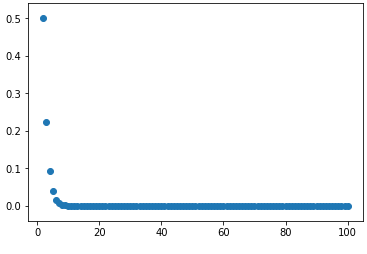
\includegraphics{clusters.png}

    4b) for K = 10 \[ 0.27\] for K = 100 \[ 5.7x10^{-7} \] for K = 1000
\[ 8.2x10^{-64}\]

7)the answer is b. More centroids should be allocated to the less dense
region.

11a) If a variable's SSE is low for all clusters than that variable is
pretty much similar for all clusters and it is useless in defining our
clustering.

11b) If the variable is low for one cluster than it is essential in
creating that cluster. Because all the points are similar in that
variable.

11c) If it's high for all clusters than that means the variable is
noise. It doesn't help in the definition of the clustering.

11d) If it is high in one cluster than that variable doesn't define that
cluster. In fact, it probably defines another clustering.

11e) By knowing the per variable SSE you can see insight into your
clustering and by identifying important variables you can cluster based
on the SSE for those variables. You can also identify variables that you
can eliminate that don't contribute to the clustering.

    \begin{enumerate}
\def\labelenumi{\arabic{enumi})}
\setcounter{enumi}{15}
\tightlist
\item
  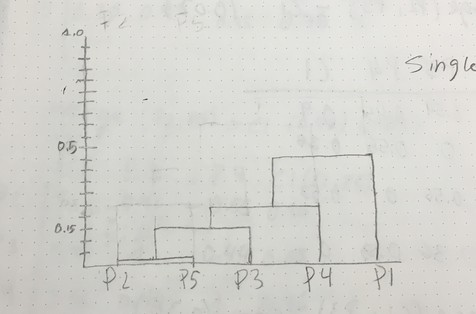
\includegraphics{IMG-2832.JPG} 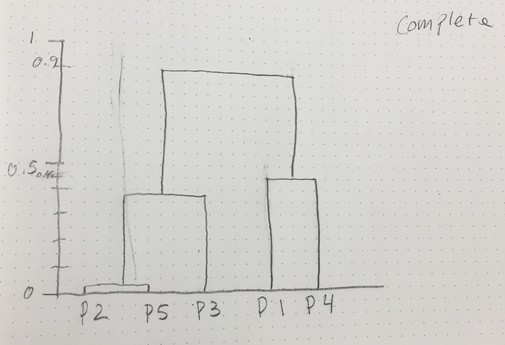
\includegraphics{complete.jpg}
\end{enumerate}

    17ai) c1 = 18, C1 = \{6, 12, 18, 24, 30\}, c2 = 45, C2 = \{42, 48\}

\begin{itemize}
\item
  SSE(C1) = \(\sum_{x\in C_1} (c_1 - x)^2\) = 360
\item
  SSE(C2) = \(\sum_{y\in C_2} (c_2 - y)^2\) = 18
\item
  total SSE = 378
\end{itemize}

17aii) c3 = 15, C3 = \{6, 12, 18, 24\}, c4 = 40, C4 = \{30, 42, 48\}

\begin{itemize}
\item
  SSE(C3) = \(\sum_{x\in C_3} (c_3 - x)^2\) = 180
\item
  SSE(C4) = \(\sum_{x\in C_4} (c_4 - x)^2\) = 168
\item
  total SSE = 348
\end{itemize}

17b) Yes the centroids are stable.

17c) C1 = \{6,12,18,24,30\} and C2 = \{42,48\}

17d) Single link produces the most natural clustering because it
preserves the structure and makes sure that the closest points are
connected together.

17e) this natural clustering is center-based.

17f) The K-Means algorithm has random intial centroids which leads to
the above behaviour of producing different clusters. Also it isn't very
good at finding clusters of different sizes.

\begin{enumerate}
\def\labelenumi{\arabic{enumi})}
\setcounter{enumi}{20}
\item
\end{enumerate}

\textbf{Entropy}

\begin{itemize}
\item
  entropy(C1) = 0.19999
\item
  entropy(C2) = 1.84075
\item
  entropy(C3) = 1.69641
\item
  total entropy = 1.44311
\end{itemize}

\textbf{Purity}

\begin{itemize}
\item
  purity(C1) = 0.97547
\item
  purity(C2) = 0.52945
\item
  purity(C3) = 0.4899895
\item
  Total purity = 0.61423
\end{itemize}

22a) There is a difference between the two sets, mainly that one will
have uniform density while the other will have regions that are more
dense and regions that are less dense.

22b) The randomly generated set will have lower SSE for K = 10. This is
because if most or all clusters are focused on the dense regions than
the overall SSE will be lower.

22c) Based on the user defined minpts and eps, DBSCAN will either put
all point in one cluster for the uniform set or label everything as
noise and eliminate it.

For the random one the DBSCAN will find a couple of clusters and based
on how the density is distributed.

\begin{enumerate}
\def\labelenumi{\arabic{enumi})}
\setcounter{enumi}{22}
\tightlist
\item
  silhoutte coefficient \(= \frac{b - a}{max(a,b)}\)
\end{enumerate}

\[ SC(P1) = \frac{\frac{0.35 + 0.45}{2} - 0.2}{max(0.2,\frac{0.35+0.45}{2})}  =  \frac{0.4 - 0.2}{max(0.2,0.4)} = 0.5\]
\[ SC(P2) = \frac{\frac{0.3 + 0.4}{2} - 0.2}{max(0.2,\frac{0.3+0.4}{2})}  =  \frac{0.35 - 0.2}{max(0.2,0.35)} = 0.42857\]
\[ SC(P3) = \frac{\frac{0.35 + 0.3}{2} - 0.1}{max(0.1,\frac{0.35+0.3}{2})}  =  \frac{0.325 - 0.1}{max(0.1,0.325)} = 0.69231\]
\[ SC(P4) = \frac{\frac{0.45 + 0.4}{2} - 0.1}{max(0.1,\frac{0.45+0.4}{2})}  =  \frac{0.425 - 0.1}{max(0.1,0.425)} = 0.76471\]
\[ SC(C1) = \frac{0.5 + 0.42857}{2} = 0.46429 \]
\[ SC(C2) = \frac{0.69231 + 0.76471}{2} = 0.72851 \]
\[ SC(Avg Clustering) = \frac{0.46429 + 0.72851}{2} = 0.5964\]

    \subsection{Practimum Problems}\label{practimum-problems}

    \begin{Verbatim}[commandchars=\\\{\}]
{\color{incolor}In [{\color{incolor}5}]:} \PY{k+kn}{import} \PY{n+nn}{numpy} \PY{k}{as} \PY{n+nn}{np}
        \PY{k+kn}{import} \PY{n+nn}{pandas} \PY{k}{as} \PY{n+nn}{pd}
        
        \PY{k+kn}{import} \PY{n+nn}{matplotlib}\PY{n+nn}{.}\PY{n+nn}{pyplot} \PY{k}{as} \PY{n+nn}{plt}
        \PY{k+kn}{import} \PY{n+nn}{seaborn} \PY{k}{as} \PY{n+nn}{sns}
        
        \PY{o}{\PYZpc{}}\PY{k}{matplotlib} inline
        
        
        \PY{k+kn}{from} \PY{n+nn}{sklearn}\PY{n+nn}{.}\PY{n+nn}{datasets} \PY{k}{import} \PY{n}{load\PYZus{}boston}
        \PY{k+kn}{from} \PY{n+nn}{sklearn}\PY{n+nn}{.}\PY{n+nn}{datasets} \PY{k}{import} \PY{n}{load\PYZus{}wine}
        \PY{k+kn}{from} \PY{n+nn}{sklearn}\PY{n+nn}{.}\PY{n+nn}{cluster} \PY{k}{import} \PY{n}{KMeans}
        
        \PY{k+kn}{from} \PY{n+nn}{sklearn} \PY{k}{import} \PY{n}{preprocessing}
        \PY{k+kn}{from} \PY{n+nn}{sklearn} \PY{k}{import} \PY{n}{metrics}
        
        \PY{k+kn}{from} \PY{n+nn}{sklearn}\PY{n+nn}{.}\PY{n+nn}{cluster} \PY{k}{import} \PY{n}{AgglomerativeClustering} \PY{k}{as} \PY{n}{ac}
\end{Verbatim}


    \paragraph{Problem 1}\label{problem-1}

Load \emph{auto-mpg} dataset from the UCI Machine Learning Repository
(auto-mpg.data) into \textbf{Python} using a Pandas dataframe. Using
only the \emph{continuous} fields as features, impute any missing values
with the \emph{mean}, and perform a Hierarchical Clustering (Use
\textbf{sklearn.cluster.AgglomerativeClustering}) with \textbf{linkage}
set to \emph{average} and the default \textbf{affinity} set to a
\emph{euclidea}. Set the remaining parameters to obtain a shallow tree
of depth 5 with 3 clusters as the target. Obtain the mean and variance
values for each cluster, and compare these values to the values obtained
for each class if we used \emph{origin} as a class label. Is there a
clear relationship between cluster assignment and class label?

    \paragraph{Answer}\label{answer}

There doesn't seem like there is any relationship between cluster
assignment and class label. The mean and variance for the attributes
varies greately between cluster assignment and class label. That being
said there are some interesting facts that show up in the clustering
data. First is that all the object of class 3 are mapped to cluster 0.
The second is that cluster 1 only has the objects from class 1. The
problem that we face with these two observations is that cluster 0
doesn't just contain class 3 so the homogenity is low and class 1 is
spread across mutliple clusters and thus there is low completeness for
class 1.

    \begin{Verbatim}[commandchars=\\\{\}]
{\color{incolor}In [{\color{incolor}6}]:} \PY{n}{auto} \PY{o}{=} \PY{n}{pd}\PY{o}{.}\PY{n}{read\PYZus{}table}\PY{p}{(}\PY{l+s+s2}{\PYZdq{}}\PY{l+s+s2}{https://archive.ics.uci.edu/ml/machine\PYZhy{}learning\PYZhy{}databases/auto\PYZhy{}mpg/auto\PYZhy{}mpg.data}\PY{l+s+s2}{\PYZdq{}}\PY{p}{,}\PY{n}{sep}\PY{o}{=}\PY{l+s+s2}{\PYZdq{}}\PY{l+s+s2}{\PYZbs{}}\PY{l+s+s2}{s+}\PY{l+s+s2}{\PYZdq{}}\PY{p}{,} \PY{n}{header}\PY{o}{=}\PY{k+kc}{None}\PY{p}{)}
        \PY{n}{auto}\PY{o}{.}\PY{n}{columns}\PY{o}{=}\PY{p}{[}\PY{l+s+s2}{\PYZdq{}}\PY{l+s+s2}{mpg}\PY{l+s+s2}{\PYZdq{}}\PY{p}{,}\PY{l+s+s2}{\PYZdq{}}\PY{l+s+s2}{cylinders}\PY{l+s+s2}{\PYZdq{}}\PY{p}{,} \PY{l+s+s2}{\PYZdq{}}\PY{l+s+s2}{displacement}\PY{l+s+s2}{\PYZdq{}}\PY{p}{,} \PY{l+s+s2}{\PYZdq{}}\PY{l+s+s2}{horsepower}\PY{l+s+s2}{\PYZdq{}}\PY{p}{,} \PY{l+s+s2}{\PYZdq{}}\PY{l+s+s2}{weight}\PY{l+s+s2}{\PYZdq{}}\PY{p}{,} \PY{l+s+s2}{\PYZdq{}}\PY{l+s+s2}{acceleration}\PY{l+s+s2}{\PYZdq{}}\PY{p}{,}\PY{l+s+s2}{\PYZdq{}}\PY{l+s+s2}{model\PYZhy{}year}\PY{l+s+s2}{\PYZdq{}}\PY{p}{,} \PY{l+s+s2}{\PYZdq{}}\PY{l+s+s2}{origin}\PY{l+s+s2}{\PYZdq{}}\PY{p}{,} \PY{l+s+s2}{\PYZdq{}}\PY{l+s+s2}{car\PYZhy{}name}\PY{l+s+s2}{\PYZdq{}}\PY{p}{]}
\end{Verbatim}


    \begin{Verbatim}[commandchars=\\\{\}]
{\color{incolor}In [{\color{incolor}7}]:} \PY{n}{auto}\PY{o}{.}\PY{n}{describe}\PY{p}{(}\PY{p}{)}
\end{Verbatim}


\begin{Verbatim}[commandchars=\\\{\}]
{\color{outcolor}Out[{\color{outcolor}7}]:}               mpg   cylinders  displacement       weight  acceleration  \textbackslash{}
        count  398.000000  398.000000    398.000000   398.000000    398.000000   
        mean    23.514573    5.454774    193.425879  2970.424623     15.568090   
        std      7.815984    1.701004    104.269838   846.841774      2.757689   
        min      9.000000    3.000000     68.000000  1613.000000      8.000000   
        25\%     17.500000    4.000000    104.250000  2223.750000     13.825000   
        50\%     23.000000    4.000000    148.500000  2803.500000     15.500000   
        75\%     29.000000    8.000000    262.000000  3608.000000     17.175000   
        max     46.600000    8.000000    455.000000  5140.000000     24.800000   
        
               model-year      origin  
        count  398.000000  398.000000  
        mean    76.010050    1.572864  
        std      3.697627    0.802055  
        min     70.000000    1.000000  
        25\%     73.000000    1.000000  
        50\%     76.000000    1.000000  
        75\%     79.000000    2.000000  
        max     82.000000    3.000000  
\end{Verbatim}
            
    \begin{Verbatim}[commandchars=\\\{\}]
{\color{incolor}In [{\color{incolor}8}]:} \PY{n}{auto}\PY{o}{.}\PY{n}{head}\PY{p}{(}\PY{p}{)}
\end{Verbatim}


\begin{Verbatim}[commandchars=\\\{\}]
{\color{outcolor}Out[{\color{outcolor}8}]:}     mpg  cylinders  displacement horsepower  weight  acceleration  model-year  \textbackslash{}
        0  18.0          8         307.0      130.0  3504.0          12.0          70   
        1  15.0          8         350.0      165.0  3693.0          11.5          70   
        2  18.0          8         318.0      150.0  3436.0          11.0          70   
        3  16.0          8         304.0      150.0  3433.0          12.0          70   
        4  17.0          8         302.0      140.0  3449.0          10.5          70   
        
           origin                   car-name  
        0       1  chevrolet chevelle malibu  
        1       1          buick skylark 320  
        2       1         plymouth satellite  
        3       1              amc rebel sst  
        4       1                ford torino  
\end{Verbatim}
            
    \begin{Verbatim}[commandchars=\\\{\}]
{\color{incolor}In [{\color{incolor}9}]:} \PY{n}{numerical} \PY{o}{=} \PY{n}{auto}\PY{o}{.}\PY{n}{drop}\PY{p}{(}\PY{n}{columns}\PY{o}{=}\PY{l+s+s2}{\PYZdq{}}\PY{l+s+s2}{car\PYZhy{}name}\PY{l+s+s2}{\PYZdq{}}\PY{p}{)}
        \PY{n}{numerical}\PY{o}{.}\PY{n}{describe}\PY{p}{(}\PY{p}{)}
\end{Verbatim}


\begin{Verbatim}[commandchars=\\\{\}]
{\color{outcolor}Out[{\color{outcolor}9}]:}               mpg   cylinders  displacement       weight  acceleration  \textbackslash{}
        count  398.000000  398.000000    398.000000   398.000000    398.000000   
        mean    23.514573    5.454774    193.425879  2970.424623     15.568090   
        std      7.815984    1.701004    104.269838   846.841774      2.757689   
        min      9.000000    3.000000     68.000000  1613.000000      8.000000   
        25\%     17.500000    4.000000    104.250000  2223.750000     13.825000   
        50\%     23.000000    4.000000    148.500000  2803.500000     15.500000   
        75\%     29.000000    8.000000    262.000000  3608.000000     17.175000   
        max     46.600000    8.000000    455.000000  5140.000000     24.800000   
        
               model-year      origin  
        count  398.000000  398.000000  
        mean    76.010050    1.572864  
        std      3.697627    0.802055  
        min     70.000000    1.000000  
        25\%     73.000000    1.000000  
        50\%     76.000000    1.000000  
        75\%     79.000000    2.000000  
        max     82.000000    3.000000  
\end{Verbatim}
            
    \begin{Verbatim}[commandchars=\\\{\}]
{\color{incolor}In [{\color{incolor}10}]:} \PY{n}{numerical}\PY{p}{[}\PY{l+s+s2}{\PYZdq{}}\PY{l+s+s2}{horsepower}\PY{l+s+s2}{\PYZdq{}}\PY{p}{]} \PY{o}{=} \PY{p}{(}\PY{n}{numerical}\PY{p}{[}\PY{l+s+s2}{\PYZdq{}}\PY{l+s+s2}{horsepower}\PY{l+s+s2}{\PYZdq{}}\PY{p}{]}\PY{o}{.}\PY{n}{replace}\PY{p}{(}\PY{n}{to\PYZus{}replace}\PY{o}{=}\PY{l+s+s2}{\PYZdq{}}\PY{l+s+s2}{?}\PY{l+s+s2}{\PYZdq{}}\PY{p}{,}\PY{n}{value}\PY{o}{=}\PY{n}{np}\PY{o}{.}\PY{n}{nan}\PY{p}{)}\PY{p}{)}\PY{o}{.}\PY{n}{astype}\PY{p}{(}\PY{n}{np}\PY{o}{.}\PY{n}{float64}\PY{p}{)}
         \PY{n}{numerical}\PY{o}{.}\PY{n}{describe}\PY{p}{(}\PY{p}{)}
\end{Verbatim}


\begin{Verbatim}[commandchars=\\\{\}]
{\color{outcolor}Out[{\color{outcolor}10}]:}               mpg   cylinders  displacement  horsepower       weight  \textbackslash{}
         count  398.000000  398.000000    398.000000  392.000000   398.000000   
         mean    23.514573    5.454774    193.425879  104.469388  2970.424623   
         std      7.815984    1.701004    104.269838   38.491160   846.841774   
         min      9.000000    3.000000     68.000000   46.000000  1613.000000   
         25\%     17.500000    4.000000    104.250000   75.000000  2223.750000   
         50\%     23.000000    4.000000    148.500000   93.500000  2803.500000   
         75\%     29.000000    8.000000    262.000000  126.000000  3608.000000   
         max     46.600000    8.000000    455.000000  230.000000  5140.000000   
         
                acceleration  model-year      origin  
         count    398.000000  398.000000  398.000000  
         mean      15.568090   76.010050    1.572864  
         std        2.757689    3.697627    0.802055  
         min        8.000000   70.000000    1.000000  
         25\%       13.825000   73.000000    1.000000  
         50\%       15.500000   76.000000    1.000000  
         75\%       17.175000   79.000000    2.000000  
         max       24.800000   82.000000    3.000000  
\end{Verbatim}
            
    \begin{Verbatim}[commandchars=\\\{\}]
{\color{incolor}In [{\color{incolor}11}]:} \PY{n}{mean\PYZus{}imp} \PY{o}{=} \PY{n}{preprocessing}\PY{o}{.}\PY{n}{Imputer}\PY{p}{(}\PY{n}{strategy}\PY{o}{=}\PY{l+s+s2}{\PYZdq{}}\PY{l+s+s2}{mean}\PY{l+s+s2}{\PYZdq{}}\PY{p}{,} \PY{n}{missing\PYZus{}values}\PY{o}{=}\PY{n}{np}\PY{o}{.}\PY{n}{nan}\PY{p}{)}
         \PY{n}{mean} \PY{o}{=} \PY{n}{mean\PYZus{}imp}\PY{o}{.}\PY{n}{fit\PYZus{}transform}\PY{p}{(}\PY{n}{numerical}\PY{o}{.}\PY{n}{drop}\PY{p}{(}\PY{n}{columns}\PY{o}{=}\PY{p}{[}\PY{l+s+s2}{\PYZdq{}}\PY{l+s+s2}{mpg}\PY{l+s+s2}{\PYZdq{}}\PY{p}{,}\PY{l+s+s2}{\PYZdq{}}\PY{l+s+s2}{cylinders}\PY{l+s+s2}{\PYZdq{}}\PY{p}{,}\PY{l+s+s2}{\PYZdq{}}\PY{l+s+s2}{displacement}\PY{l+s+s2}{\PYZdq{}}\PY{p}{,}
                                                               \PY{l+s+s2}{\PYZdq{}}\PY{l+s+s2}{weight}\PY{l+s+s2}{\PYZdq{}}\PY{p}{,}\PY{l+s+s2}{\PYZdq{}}\PY{l+s+s2}{acceleration}\PY{l+s+s2}{\PYZdq{}}\PY{p}{,}\PY{l+s+s2}{\PYZdq{}}\PY{l+s+s2}{model\PYZhy{}year}\PY{l+s+s2}{\PYZdq{}}\PY{p}{,}\PY{l+s+s2}{\PYZdq{}}\PY{l+s+s2}{origin}\PY{l+s+s2}{\PYZdq{}}\PY{p}{]}\PY{p}{)}\PY{p}{)}
         \PY{n}{numerical}\PY{p}{[}\PY{l+s+s2}{\PYZdq{}}\PY{l+s+s2}{horsepower}\PY{l+s+s2}{\PYZdq{}}\PY{p}{]} \PY{o}{=} \PY{n}{mean}
         \PY{n}{numerical}\PY{o}{.}\PY{n}{describe}\PY{p}{(}\PY{p}{)}
\end{Verbatim}


    \begin{Verbatim}[commandchars=\\\{\}]
/home/mahmoud/anaconda3/lib/python3.6/site-packages/sklearn/utils/deprecation.py:58: DeprecationWarning: Class Imputer is deprecated; Imputer was deprecated in version 0.20 and will be removed in 0.22. Import impute.SimpleImputer from sklearn instead.
  warnings.warn(msg, category=DeprecationWarning)

    \end{Verbatim}

\begin{Verbatim}[commandchars=\\\{\}]
{\color{outcolor}Out[{\color{outcolor}11}]:}               mpg   cylinders  displacement  horsepower       weight  \textbackslash{}
         count  398.000000  398.000000    398.000000  398.000000   398.000000   
         mean    23.514573    5.454774    193.425879  104.469388  2970.424623   
         std      7.815984    1.701004    104.269838   38.199187   846.841774   
         min      9.000000    3.000000     68.000000   46.000000  1613.000000   
         25\%     17.500000    4.000000    104.250000   76.000000  2223.750000   
         50\%     23.000000    4.000000    148.500000   95.000000  2803.500000   
         75\%     29.000000    8.000000    262.000000  125.000000  3608.000000   
         max     46.600000    8.000000    455.000000  230.000000  5140.000000   
         
                acceleration  model-year      origin  
         count    398.000000  398.000000  398.000000  
         mean      15.568090   76.010050    1.572864  
         std        2.757689    3.697627    0.802055  
         min        8.000000   70.000000    1.000000  
         25\%       13.825000   73.000000    1.000000  
         50\%       15.500000   76.000000    1.000000  
         75\%       17.175000   79.000000    2.000000  
         max       24.800000   82.000000    3.000000  
\end{Verbatim}
            
    \begin{Verbatim}[commandchars=\\\{\}]
{\color{incolor}In [{\color{incolor}12}]:} \PY{n}{numerical}\PY{o}{.}\PY{n}{head}\PY{p}{(}\PY{p}{)}
\end{Verbatim}


\begin{Verbatim}[commandchars=\\\{\}]
{\color{outcolor}Out[{\color{outcolor}12}]:}     mpg  cylinders  displacement  horsepower  weight  acceleration  \textbackslash{}
         0  18.0          8         307.0       130.0  3504.0          12.0   
         1  15.0          8         350.0       165.0  3693.0          11.5   
         2  18.0          8         318.0       150.0  3436.0          11.0   
         3  16.0          8         304.0       150.0  3433.0          12.0   
         4  17.0          8         302.0       140.0  3449.0          10.5   
         
            model-year  origin  
         0          70       1  
         1          70       1  
         2          70       1  
         3          70       1  
         4          70       1  
\end{Verbatim}
            
    \begin{Verbatim}[commandchars=\\\{\}]
{\color{incolor}In [{\color{incolor}13}]:} \PY{n}{clust} \PY{o}{=} \PY{n}{ac}\PY{p}{(}\PY{n}{linkage}\PY{o}{=}\PY{l+s+s2}{\PYZdq{}}\PY{l+s+s2}{average}\PY{l+s+s2}{\PYZdq{}}\PY{p}{,} \PY{n}{n\PYZus{}clusters}\PY{o}{=}\PY{l+m+mi}{3}\PY{p}{,} \PY{n}{compute\PYZus{}full\PYZus{}tree}\PY{o}{=}\PY{k+kc}{False}\PY{p}{)}
         \PY{n}{auto\PYZus{}cluster} \PY{o}{=} \PY{n}{clust}\PY{o}{.}\PY{n}{fit}\PY{p}{(}\PY{n}{numerical}\PY{p}{)}
         \PY{n}{numerical}\PY{p}{[}\PY{l+s+s2}{\PYZdq{}}\PY{l+s+s2}{Clust label}\PY{l+s+s2}{\PYZdq{}}\PY{p}{]} \PY{o}{=} \PY{n}{auto\PYZus{}cluster}\PY{o}{.}\PY{n}{labels\PYZus{}}
         \PY{n+nb}{print}\PY{p}{(}\PY{n}{auto\PYZus{}cluster}\PY{o}{.}\PY{n}{labels\PYZus{}}\PY{p}{)}
\end{Verbatim}


    \begin{Verbatim}[commandchars=\\\{\}]
[2 2 2 2 2 1 1 1 1 2 2 2 2 0 0 0 0 0 0 0 0 0 0 0 0 1 1 1 1 0 0 0 0 0 2 2 0
 0 1 1 1 1 1 1 1 0 0 0 0 0 0 0 0 0 0 0 0 0 0 0 0 0 1 1 1 1 2 1 1 1 1 0 2 1
 1 1 0 0 0 0 0 0 0 0 0 1 2 2 1 2 1 1 1 1 1 1 2 0 0 0 0 0 0 1 1 1 1 0 0 0 0
 0 0 0 0 1 1 0 0 0 0 2 0 0 2 0 0 0 2 0 0 0 0 2 2 2 1 1 1 1 1 0 0 0 0 0 0 0
 0 0 0 0 0 2 2 0 1 1 1 1 2 2 2 2 0 0 0 0 0 0 0 0 0 0 0 0 0 0 0 0 0 0 0 0 0
 0 0 1 1 2 1 0 2 0 0 0 0 0 0 2 2 2 0 0 0 0 0 0 2 0 0 2 1 1 2 2 0 0 0 0 0 2
 1 1 1 2 2 2 2 1 1 1 1 0 0 0 0 0 0 0 0 0 0 0 0 0 0 0 0 2 2 2 2 0 0 0 2 0 2
 0 2 2 2 2 0 1 0 0 0 0 0 0 0 0 0 0 0 2 0 0 0 0 0 0 2 2 2 2 2 1 1 2 2 0 0 0
 0 2 2 0 2 0 0 0 0 0 0 0 0 0 0 0 0 0 0 0 2 0 0 0 0 0 0 0 0 0 0 0 0 0 0 0 0
 0 0 0 0 0 0 0 0 0 0 0 0 0 0 0 0 0 0 0 0 0 0 0 0 0 0 0 0 0 0 2 2 0 2 0 0 0
 0 0 0 0 0 0 0 0 0 0 0 0 0 0 0 0 0 0 0 0 0 0 0 0 0 0 0 0]

    \end{Verbatim}

    \begin{Verbatim}[commandchars=\\\{\}]
{\color{incolor}In [{\color{incolor}14}]:} \PY{n}{numerical}\PY{o}{.}\PY{n}{describe}\PY{p}{(}\PY{p}{)}
\end{Verbatim}


\begin{Verbatim}[commandchars=\\\{\}]
{\color{outcolor}Out[{\color{outcolor}14}]:}               mpg   cylinders  displacement  horsepower       weight  \textbackslash{}
         count  398.000000  398.000000    398.000000  398.000000   398.000000   
         mean    23.514573    5.454774    193.425879  104.469388  2970.424623   
         std      7.815984    1.701004    104.269838   38.199187   846.841774   
         min      9.000000    3.000000     68.000000   46.000000  1613.000000   
         25\%     17.500000    4.000000    104.250000   76.000000  2223.750000   
         50\%     23.000000    4.000000    148.500000   95.000000  2803.500000   
         75\%     29.000000    8.000000    262.000000  125.000000  3608.000000   
         max     46.600000    8.000000    455.000000  230.000000  5140.000000   
         
                acceleration  model-year      origin  Clust label  
         count    398.000000  398.000000  398.000000   398.000000  
         mean      15.568090   76.010050    1.572864     0.502513  
         std        2.757689    3.697627    0.802055     0.770190  
         min        8.000000   70.000000    1.000000     0.000000  
         25\%       13.825000   73.000000    1.000000     0.000000  
         50\%       15.500000   76.000000    1.000000     0.000000  
         75\%       17.175000   79.000000    2.000000     1.000000  
         max       24.800000   82.000000    3.000000     2.000000  
\end{Verbatim}
            
    \begin{Verbatim}[commandchars=\\\{\}]
{\color{incolor}In [{\color{incolor}15}]:} \PY{n}{numerical}\PY{p}{[}\PY{l+s+s2}{\PYZdq{}}\PY{l+s+s2}{origin}\PY{l+s+s2}{\PYZdq{}}\PY{p}{]}\PY{o}{.}\PY{n}{unique}\PY{p}{(}\PY{p}{)}
\end{Verbatim}


\begin{Verbatim}[commandchars=\\\{\}]
{\color{outcolor}Out[{\color{outcolor}15}]:} array([1, 3, 2])
\end{Verbatim}
            
    \begin{Verbatim}[commandchars=\\\{\}]
{\color{incolor}In [{\color{incolor}16}]:} \PY{n}{class\PYZus{}origin} \PY{o}{=} \PY{p}{[}\PY{p}{]}
         \PY{n}{class\PYZus{}origin}\PY{o}{.}\PY{n}{append}\PY{p}{(}\PY{n}{numerical}\PY{p}{[}\PY{n}{numerical}\PY{p}{[}\PY{l+s+s2}{\PYZdq{}}\PY{l+s+s2}{origin}\PY{l+s+s2}{\PYZdq{}}\PY{p}{]} \PY{o}{==} \PY{l+m+mi}{1}\PY{p}{]}\PY{p}{)}
         \PY{n}{class\PYZus{}origin}\PY{o}{.}\PY{n}{append}\PY{p}{(}\PY{n}{numerical}\PY{p}{[}\PY{n}{numerical}\PY{p}{[}\PY{l+s+s2}{\PYZdq{}}\PY{l+s+s2}{origin}\PY{l+s+s2}{\PYZdq{}}\PY{p}{]} \PY{o}{==} \PY{l+m+mi}{2}\PY{p}{]}\PY{p}{)}
         \PY{n}{class\PYZus{}origin}\PY{o}{.}\PY{n}{append}\PY{p}{(}\PY{n}{numerical}\PY{p}{[}\PY{n}{numerical}\PY{p}{[}\PY{l+s+s2}{\PYZdq{}}\PY{l+s+s2}{origin}\PY{l+s+s2}{\PYZdq{}}\PY{p}{]} \PY{o}{==} \PY{l+m+mi}{3}\PY{p}{]}\PY{p}{)}
         \PY{n}{class\PYZus{}origin}\PY{p}{[}\PY{l+m+mi}{0}\PY{p}{]}\PY{o}{.}\PY{n}{describe}\PY{p}{(}\PY{p}{)}
\end{Verbatim}


\begin{Verbatim}[commandchars=\\\{\}]
{\color{outcolor}Out[{\color{outcolor}16}]:}               mpg   cylinders  displacement  horsepower       weight  \textbackslash{}
         count  249.000000  249.000000    249.000000  249.000000   249.000000   
         mean    20.083534    6.248996    245.901606  118.814769  3361.931727   
         std      6.402892    1.661425     98.501839   39.617323   794.792506   
         min      9.000000    4.000000     85.000000   52.000000  1800.000000   
         25\%     15.000000    4.000000    151.000000   88.000000  2720.000000   
         50\%     18.500000    6.000000    250.000000  105.000000  3365.000000   
         75\%     24.000000    8.000000    318.000000  150.000000  4054.000000   
         max     39.000000    8.000000    455.000000  230.000000  5140.000000   
         
                acceleration  model-year  origin  Clust label  
         count    249.000000  249.000000   249.0   249.000000  
         mean      15.033735   75.610442     1.0     0.779116  
         std        2.751112    3.677094     0.0     0.834854  
         min        8.000000   70.000000     1.0     0.000000  
         25\%       13.000000   73.000000     1.0     0.000000  
         50\%       15.000000   76.000000     1.0     1.000000  
         75\%       16.900000   79.000000     1.0     2.000000  
         max       22.200000   82.000000     1.0     2.000000  
\end{Verbatim}
            
    \begin{Verbatim}[commandchars=\\\{\}]
{\color{incolor}In [{\color{incolor}17}]:} \PY{n}{clust} \PY{o}{=} \PY{p}{[}\PY{p}{]}
         \PY{n}{clust}\PY{o}{.}\PY{n}{append}\PY{p}{(}\PY{n}{numerical}\PY{p}{[}\PY{n}{numerical}\PY{p}{[}\PY{l+s+s2}{\PYZdq{}}\PY{l+s+s2}{Clust label}\PY{l+s+s2}{\PYZdq{}}\PY{p}{]} \PY{o}{==} \PY{l+m+mi}{0}\PY{p}{]}\PY{p}{)}
         \PY{n}{clust}\PY{o}{.}\PY{n}{append}\PY{p}{(}\PY{n}{numerical}\PY{p}{[}\PY{n}{numerical}\PY{p}{[}\PY{l+s+s2}{\PYZdq{}}\PY{l+s+s2}{Clust label}\PY{l+s+s2}{\PYZdq{}}\PY{p}{]} \PY{o}{==} \PY{l+m+mi}{1}\PY{p}{]}\PY{p}{)}
         \PY{n}{clust}\PY{o}{.}\PY{n}{append}\PY{p}{(}\PY{n}{numerical}\PY{p}{[}\PY{n}{numerical}\PY{p}{[}\PY{l+s+s2}{\PYZdq{}}\PY{l+s+s2}{Clust label}\PY{l+s+s2}{\PYZdq{}}\PY{p}{]} \PY{o}{==} \PY{l+m+mi}{2}\PY{p}{]}\PY{p}{)}
         \PY{n}{clust}\PY{p}{[}\PY{l+m+mi}{0}\PY{p}{]}\PY{o}{.}\PY{n}{describe}\PY{p}{(}\PY{p}{)}
\end{Verbatim}


\begin{Verbatim}[commandchars=\\\{\}]
{\color{outcolor}Out[{\color{outcolor}17}]:}               mpg   cylinders  displacement  horsepower       weight  \textbackslash{}
         count  266.000000  266.000000    266.000000  266.000000   266.000000   
         mean    27.365414    4.443609    131.934211   84.300061  2459.511278   
         std      6.478913    0.922781     53.179727   19.213107   427.354771   
         min     13.000000    3.000000     68.000000   46.000000  1613.000000   
         25\%     22.075000    4.000000     97.000000   70.000000  2124.250000   
         50\%     26.900000    4.000000    119.000000   85.000000  2395.000000   
         75\%     32.000000    4.000000    149.750000   95.000000  2805.250000   
         max     46.600000    8.000000    455.000000  225.000000  3302.000000   
         
                acceleration  model-year      origin  Clust label  
         count    266.000000  266.000000  266.000000        266.0  
         mean      16.298120   76.751880    1.845865          0.0  
         std        2.391296    3.760582    0.852699          0.0  
         min       10.000000   70.000000    1.000000          0.0  
         25\%       14.550000   74.000000    1.000000          0.0  
         50\%       16.000000   77.000000    2.000000          0.0  
         75\%       17.600000   80.000000    3.000000          0.0  
         max       24.800000   82.000000    3.000000          0.0  
\end{Verbatim}
            
    \begin{Verbatim}[commandchars=\\\{\}]
{\color{incolor}In [{\color{incolor}18}]:} \PY{n}{clust}\PY{p}{[}\PY{l+m+mi}{1}\PY{p}{]}\PY{o}{.}\PY{n}{describe}\PY{p}{(}\PY{p}{)}
\end{Verbatim}


\begin{Verbatim}[commandchars=\\\{\}]
{\color{outcolor}Out[{\color{outcolor}18}]:}              mpg  cylinders  displacement  horsepower       weight  \textbackslash{}
         count  64.000000       64.0     64.000000   64.000000    64.000000   
         mean   13.889062        8.0    358.093750  167.046875  4398.593750   
         std     1.832781        0.0     46.240818   27.504937   272.602899   
         min     9.000000        8.0    260.000000  110.000000  4042.000000   
         25\%    13.000000        8.0    318.000000  149.750000  4183.750000   
         50\%    14.000000        8.0    350.000000  156.500000  4357.000000   
         75\%    15.125000        8.0    400.000000  180.000000  4530.250000   
         max    17.500000        8.0    455.000000  230.000000  5140.000000   
         
                acceleration  model-year  origin  Clust label  
         count     64.000000   64.000000    64.0         64.0  
         mean      13.025000   73.375000     1.0          1.0  
         std        1.895106    2.446248     0.0          0.0  
         min        8.500000   70.000000     1.0          1.0  
         25\%       12.000000   72.000000     1.0          1.0  
         50\%       13.000000   73.000000     1.0          1.0  
         75\%       14.000000   75.000000     1.0          1.0  
         max       19.000000   79.000000     1.0          1.0  
\end{Verbatim}
            
    \begin{Verbatim}[commandchars=\\\{\}]
{\color{incolor}In [{\color{incolor}19}]:} \PY{n}{clust}\PY{p}{[}\PY{l+m+mi}{2}\PY{p}{]}\PY{o}{.}\PY{n}{describe}\PY{p}{(}\PY{p}{)}
\end{Verbatim}


\begin{Verbatim}[commandchars=\\\{\}]
{\color{outcolor}Out[{\color{outcolor}19}]:}              mpg  cylinders  displacement  horsepower       weight  \textbackslash{}
         count  68.000000  68.000000     68.000000   68.000000    68.000000   
         mean   17.510294   7.014706    278.985294  124.470588  3624.838235   
         std     2.971513   1.029311     53.688847   26.703720   194.359999   
         min    11.000000   5.000000    163.000000   72.000000  3329.000000   
         25\%    15.000000   6.000000    231.000000  105.000000  3435.250000   
         50\%    17.550000   8.000000    260.000000  120.000000  3616.500000   
         75\%    19.125000   8.000000    318.000000  150.000000  3782.000000   
         max    26.600000   8.000000    400.000000  190.000000  3988.000000   
         
                acceleration  model-year     origin  Clust label  
         count     68.000000   68.000000  68.000000         68.0  
         mean      15.105882   75.588235   1.044118          2.0  
         std        3.249151    3.233386   0.206883          0.0  
         min        8.000000   70.000000   1.000000          2.0  
         25\%       12.725000   73.000000   1.000000          2.0  
         50\%       15.450000   76.000000   1.000000          2.0  
         75\%       17.250000   78.000000   1.000000          2.0  
         max       22.200000   81.000000   2.000000          2.0  
\end{Verbatim}
            
    \begin{Verbatim}[commandchars=\\\{\}]
{\color{incolor}In [{\color{incolor}20}]:} \PY{n+nb}{print}\PY{p}{(}\PY{l+s+s2}{\PYZdq{}}\PY{l+s+s2}{Origin 1 mean}\PY{l+s+s2}{\PYZdq{}}\PY{p}{)}
         \PY{n+nb}{print}\PY{p}{(}\PY{n}{class\PYZus{}origin}\PY{p}{[}\PY{l+m+mi}{0}\PY{p}{]}\PY{o}{.}\PY{n}{mean}\PY{p}{(}\PY{p}{)}\PY{p}{)}
         \PY{n+nb}{print}\PY{p}{(}\PY{p}{)}
         \PY{n+nb}{print}\PY{p}{(}\PY{l+s+s2}{\PYZdq{}}\PY{l+s+s2}{Origin 2 mean}\PY{l+s+s2}{\PYZdq{}}\PY{p}{)}
         \PY{n+nb}{print}\PY{p}{(}\PY{n}{class\PYZus{}origin}\PY{p}{[}\PY{l+m+mi}{1}\PY{p}{]}\PY{o}{.}\PY{n}{mean}\PY{p}{(}\PY{p}{)}\PY{p}{)}
         \PY{n+nb}{print}\PY{p}{(}\PY{p}{)}
         \PY{n+nb}{print}\PY{p}{(}\PY{l+s+s2}{\PYZdq{}}\PY{l+s+s2}{Origin 3 mean}\PY{l+s+s2}{\PYZdq{}}\PY{p}{)}
         \PY{n+nb}{print}\PY{p}{(}\PY{n}{class\PYZus{}origin}\PY{p}{[}\PY{l+m+mi}{2}\PY{p}{]}\PY{o}{.}\PY{n}{mean}\PY{p}{(}\PY{p}{)}\PY{p}{)}
\end{Verbatim}


    \begin{Verbatim}[commandchars=\\\{\}]
Origin 1 mean
mpg               20.083534
cylinders          6.248996
displacement     245.901606
horsepower       118.814769
weight          3361.931727
acceleration      15.033735
model-year        75.610442
origin             1.000000
Clust label        0.779116
dtype: float64

Origin 2 mean
mpg               27.891429
cylinders          4.157143
displacement     109.142857
horsepower        81.241983
weight          2423.300000
acceleration      16.787143
model-year        75.814286
origin             2.000000
Clust label        0.085714
dtype: float64

Origin 3 mean
mpg               30.450633
cylinders          4.101266
displacement     102.708861
horsepower        79.835443
weight          2221.227848
acceleration      16.172152
model-year        77.443038
origin             3.000000
Clust label        0.000000
dtype: float64

    \end{Verbatim}

    \begin{Verbatim}[commandchars=\\\{\}]
{\color{incolor}In [{\color{incolor}22}]:} \PY{n+nb}{print}\PY{p}{(}\PY{l+s+s2}{\PYZdq{}}\PY{l+s+s2}{Cluster 0 mean}\PY{l+s+s2}{\PYZdq{}}\PY{p}{)}
         \PY{n+nb}{print}\PY{p}{(}\PY{n}{clust}\PY{p}{[}\PY{l+m+mi}{0}\PY{p}{]}\PY{o}{.}\PY{n}{mean}\PY{p}{(}\PY{p}{)}\PY{p}{)}
         \PY{n+nb}{print}\PY{p}{(}\PY{p}{)}
         \PY{n+nb}{print}\PY{p}{(}\PY{l+s+s2}{\PYZdq{}}\PY{l+s+s2}{Cluster 1 mean}\PY{l+s+s2}{\PYZdq{}}\PY{p}{)}
         \PY{n+nb}{print}\PY{p}{(}\PY{n}{clust}\PY{p}{[}\PY{l+m+mi}{1}\PY{p}{]}\PY{o}{.}\PY{n}{mean}\PY{p}{(}\PY{p}{)}\PY{p}{)}
         \PY{n+nb}{print}\PY{p}{(}\PY{p}{)}
         \PY{n+nb}{print}\PY{p}{(}\PY{l+s+s2}{\PYZdq{}}\PY{l+s+s2}{Cluster 2 mean}\PY{l+s+s2}{\PYZdq{}}\PY{p}{)}
         \PY{n+nb}{print}\PY{p}{(}\PY{n}{clust}\PY{p}{[}\PY{l+m+mi}{2}\PY{p}{]}\PY{o}{.}\PY{n}{mean}\PY{p}{(}\PY{p}{)}\PY{p}{)}
\end{Verbatim}


    \begin{Verbatim}[commandchars=\\\{\}]
Cluster 0 mean
mpg               27.365414
cylinders          4.443609
displacement     131.934211
horsepower        84.300061
weight          2459.511278
acceleration      16.298120
model-year        76.751880
origin             1.845865
Clust label        0.000000
dtype: float64

Cluster 1 mean
mpg               13.889062
cylinders          8.000000
displacement     358.093750
horsepower       167.046875
weight          4398.593750
acceleration      13.025000
model-year        73.375000
origin             1.000000
Clust label        1.000000
dtype: float64

Cluster 2 mean
mpg               17.510294
cylinders          7.014706
displacement     278.985294
horsepower       124.470588
weight          3624.838235
acceleration      15.105882
model-year        75.588235
origin             1.044118
Clust label        2.000000
dtype: float64

    \end{Verbatim}

    \begin{Verbatim}[commandchars=\\\{\}]
{\color{incolor}In [{\color{incolor}28}]:} \PY{n+nb}{print}\PY{p}{(}\PY{l+s+s2}{\PYZdq{}}\PY{l+s+s2}{Difference mean 00}\PY{l+s+s2}{\PYZdq{}}\PY{p}{)}
         \PY{n}{m00} \PY{o}{=} \PY{n}{class\PYZus{}origin}\PY{p}{[}\PY{l+m+mi}{0}\PY{p}{]}\PY{o}{.}\PY{n}{mean}\PY{p}{(}\PY{p}{)}\PY{o}{\PYZhy{}}\PY{n}{clust}\PY{p}{[}\PY{l+m+mi}{0}\PY{p}{]}\PY{o}{.}\PY{n}{mean}\PY{p}{(}\PY{p}{)}
         \PY{n+nb}{print}\PY{p}{(}\PY{n}{m00}\PY{p}{)}
         \PY{n+nb}{print}\PY{p}{(}\PY{p}{)}
         \PY{n+nb}{print}\PY{p}{(}\PY{l+s+s2}{\PYZdq{}}\PY{l+s+s2}{Difference mean 01}\PY{l+s+s2}{\PYZdq{}}\PY{p}{)}
         \PY{n}{m01} \PY{o}{=} \PY{n}{class\PYZus{}origin}\PY{p}{[}\PY{l+m+mi}{0}\PY{p}{]}\PY{o}{.}\PY{n}{mean}\PY{p}{(}\PY{p}{)}\PY{o}{\PYZhy{}}\PY{n}{clust}\PY{p}{[}\PY{l+m+mi}{1}\PY{p}{]}\PY{o}{.}\PY{n}{mean}\PY{p}{(}\PY{p}{)}
         \PY{n+nb}{print}\PY{p}{(}\PY{n}{m01}\PY{p}{)}
         \PY{n+nb}{print}\PY{p}{(}\PY{p}{)}
         \PY{n+nb}{print}\PY{p}{(}\PY{l+s+s2}{\PYZdq{}}\PY{l+s+s2}{Difference mean 02}\PY{l+s+s2}{\PYZdq{}}\PY{p}{)}
         \PY{n}{m02} \PY{o}{=} \PY{n}{class\PYZus{}origin}\PY{p}{[}\PY{l+m+mi}{0}\PY{p}{]}\PY{o}{.}\PY{n}{mean}\PY{p}{(}\PY{p}{)}\PY{o}{\PYZhy{}}\PY{n}{clust}\PY{p}{[}\PY{l+m+mi}{2}\PY{p}{]}\PY{o}{.}\PY{n}{mean}\PY{p}{(}\PY{p}{)}
         \PY{n+nb}{print}\PY{p}{(}\PY{n}{m02}\PY{p}{)}
\end{Verbatim}


    \begin{Verbatim}[commandchars=\\\{\}]
Difference mean 00
mpg              -7.281879
cylinders         1.805387
displacement    113.967396
horsepower       34.514708
weight          902.420449
acceleration     -1.264385
model-year       -1.141438
origin           -0.845865
Clust label       0.779116
dtype: float64

Difference mean 01
mpg                6.194472
cylinders         -1.751004
displacement    -112.192144
horsepower       -48.232106
weight         -1036.662023
acceleration       2.008735
model-year         2.235442
origin             0.000000
Clust label       -0.220884
dtype: float64

Difference mean 02
mpg               2.573240
cylinders        -0.765710
displacement    -33.083688
horsepower       -5.655819
weight         -262.906508
acceleration     -0.072147
model-year        0.022206
origin           -0.044118
Clust label      -1.220884
dtype: float64

    \end{Verbatim}

    \begin{Verbatim}[commandchars=\\\{\}]
{\color{incolor}In [{\color{incolor}29}]:} \PY{n+nb}{print}\PY{p}{(}\PY{l+s+s2}{\PYZdq{}}\PY{l+s+s2}{Difference mean 10}\PY{l+s+s2}{\PYZdq{}}\PY{p}{)}
         \PY{n}{m10} \PY{o}{=} \PY{n}{class\PYZus{}origin}\PY{p}{[}\PY{l+m+mi}{1}\PY{p}{]}\PY{o}{.}\PY{n}{mean}\PY{p}{(}\PY{p}{)}\PY{o}{\PYZhy{}}\PY{n}{clust}\PY{p}{[}\PY{l+m+mi}{0}\PY{p}{]}\PY{o}{.}\PY{n}{mean}\PY{p}{(}\PY{p}{)}
         \PY{n+nb}{print}\PY{p}{(}\PY{n}{m10}\PY{p}{)}
         \PY{n+nb}{print}\PY{p}{(}\PY{p}{)}
         \PY{n+nb}{print}\PY{p}{(}\PY{l+s+s2}{\PYZdq{}}\PY{l+s+s2}{Difference mean 11}\PY{l+s+s2}{\PYZdq{}}\PY{p}{)}
         \PY{n}{m11} \PY{o}{=} \PY{n}{class\PYZus{}origin}\PY{p}{[}\PY{l+m+mi}{1}\PY{p}{]}\PY{o}{.}\PY{n}{mean}\PY{p}{(}\PY{p}{)}\PY{o}{\PYZhy{}}\PY{n}{clust}\PY{p}{[}\PY{l+m+mi}{1}\PY{p}{]}\PY{o}{.}\PY{n}{mean}\PY{p}{(}\PY{p}{)}
         \PY{n+nb}{print}\PY{p}{(}\PY{n}{m11}\PY{p}{)}
         \PY{n+nb}{print}\PY{p}{(}\PY{p}{)}
         \PY{n+nb}{print}\PY{p}{(}\PY{l+s+s2}{\PYZdq{}}\PY{l+s+s2}{Difference mean 12}\PY{l+s+s2}{\PYZdq{}}\PY{p}{)}
         \PY{n}{m12} \PY{o}{=} \PY{n}{class\PYZus{}origin}\PY{p}{[}\PY{l+m+mi}{1}\PY{p}{]}\PY{o}{.}\PY{n}{mean}\PY{p}{(}\PY{p}{)}\PY{o}{\PYZhy{}}\PY{n}{clust}\PY{p}{[}\PY{l+m+mi}{2}\PY{p}{]}\PY{o}{.}\PY{n}{mean}\PY{p}{(}\PY{p}{)}
         \PY{n+nb}{print}\PY{p}{(}\PY{n}{m12}\PY{p}{)}
\end{Verbatim}


    \begin{Verbatim}[commandchars=\\\{\}]
Difference mean 10
mpg              0.526015
cylinders       -0.286466
displacement   -22.791353
horsepower      -3.058079
weight         -36.211278
acceleration     0.489023
model-year      -0.937594
origin           0.154135
Clust label      0.085714
dtype: float64

Difference mean 11
mpg               14.002366
cylinders         -3.842857
displacement    -248.950893
horsepower       -85.804892
weight         -1975.293750
acceleration       3.762143
model-year         2.439286
origin             1.000000
Clust label       -0.914286
dtype: float64

Difference mean 12
mpg               10.381134
cylinders         -2.857563
displacement    -169.842437
horsepower       -43.228606
weight         -1201.538235
acceleration       1.681261
model-year         0.226050
origin             0.955882
Clust label       -1.914286
dtype: float64

    \end{Verbatim}

    \begin{Verbatim}[commandchars=\\\{\}]
{\color{incolor}In [{\color{incolor}30}]:} \PY{n+nb}{print}\PY{p}{(}\PY{l+s+s2}{\PYZdq{}}\PY{l+s+s2}{Difference mean 20}\PY{l+s+s2}{\PYZdq{}}\PY{p}{)}
         \PY{n}{m20} \PY{o}{=} \PY{n}{class\PYZus{}origin}\PY{p}{[}\PY{l+m+mi}{2}\PY{p}{]}\PY{o}{.}\PY{n}{mean}\PY{p}{(}\PY{p}{)}\PY{o}{\PYZhy{}}\PY{n}{clust}\PY{p}{[}\PY{l+m+mi}{0}\PY{p}{]}\PY{o}{.}\PY{n}{mean}\PY{p}{(}\PY{p}{)}
         \PY{n+nb}{print}\PY{p}{(}\PY{n}{m20}\PY{p}{)}
         \PY{n+nb}{print}\PY{p}{(}\PY{p}{)}
         \PY{n+nb}{print}\PY{p}{(}\PY{l+s+s2}{\PYZdq{}}\PY{l+s+s2}{Difference mean 21}\PY{l+s+s2}{\PYZdq{}}\PY{p}{)}
         \PY{n}{m21} \PY{o}{=} \PY{n}{class\PYZus{}origin}\PY{p}{[}\PY{l+m+mi}{2}\PY{p}{]}\PY{o}{.}\PY{n}{mean}\PY{p}{(}\PY{p}{)}\PY{o}{\PYZhy{}}\PY{n}{clust}\PY{p}{[}\PY{l+m+mi}{1}\PY{p}{]}\PY{o}{.}\PY{n}{mean}\PY{p}{(}\PY{p}{)}
         \PY{n+nb}{print}\PY{p}{(}\PY{n}{m21}\PY{p}{)}
         \PY{n+nb}{print}\PY{p}{(}\PY{p}{)}
         \PY{n+nb}{print}\PY{p}{(}\PY{l+s+s2}{\PYZdq{}}\PY{l+s+s2}{Difference mean 22}\PY{l+s+s2}{\PYZdq{}}\PY{p}{)}
         \PY{n}{m22} \PY{o}{=} \PY{n}{class\PYZus{}origin}\PY{p}{[}\PY{l+m+mi}{2}\PY{p}{]}\PY{o}{.}\PY{n}{mean}\PY{p}{(}\PY{p}{)}\PY{o}{\PYZhy{}}\PY{n}{clust}\PY{p}{[}\PY{l+m+mi}{2}\PY{p}{]}\PY{o}{.}\PY{n}{mean}\PY{p}{(}\PY{p}{)}
         \PY{n+nb}{print}\PY{p}{(}\PY{n}{m22}\PY{p}{)}
\end{Verbatim}


    \begin{Verbatim}[commandchars=\\\{\}]
Difference mean 20
mpg               3.085219
cylinders        -0.342343
displacement    -29.225350
horsepower       -4.464618
weight         -238.283430
acceleration     -0.125968
model-year        0.691158
origin            1.154135
Clust label       0.000000
dtype: float64

Difference mean 21
mpg               16.561570
cylinders         -3.898734
displacement    -255.384889
horsepower       -87.211432
weight         -2177.365902
acceleration       3.147152
model-year         4.068038
origin             2.000000
Clust label       -1.000000
dtype: float64

Difference mean 22
mpg               12.940339
cylinders         -2.913440
displacement    -176.276433
horsepower       -44.635145
weight         -1403.610387
acceleration       1.066270
model-year         1.854803
origin             1.955882
Clust label       -2.000000
dtype: float64

    \end{Verbatim}

    \begin{Verbatim}[commandchars=\\\{\}]
{\color{incolor}In [{\color{incolor}32}]:} \PY{n+nb}{print}\PY{p}{(}\PY{l+s+s2}{\PYZdq{}}\PY{l+s+s2}{Cluster 0 variance}\PY{l+s+s2}{\PYZdq{}}\PY{p}{)}
         \PY{n+nb}{print}\PY{p}{(}\PY{n}{clust}\PY{p}{[}\PY{l+m+mi}{0}\PY{p}{]}\PY{o}{.}\PY{n}{var}\PY{p}{(}\PY{p}{)}\PY{p}{)}
         \PY{n+nb}{print}\PY{p}{(}\PY{p}{)}
         \PY{n+nb}{print}\PY{p}{(}\PY{l+s+s2}{\PYZdq{}}\PY{l+s+s2}{Cluster 1 variance}\PY{l+s+s2}{\PYZdq{}}\PY{p}{)}
         \PY{n+nb}{print}\PY{p}{(}\PY{n}{clust}\PY{p}{[}\PY{l+m+mi}{1}\PY{p}{]}\PY{o}{.}\PY{n}{var}\PY{p}{(}\PY{p}{)}\PY{p}{)}
         \PY{n+nb}{print}\PY{p}{(}\PY{p}{)}
         \PY{n+nb}{print}\PY{p}{(}\PY{l+s+s2}{\PYZdq{}}\PY{l+s+s2}{Cluster 2 variance}\PY{l+s+s2}{\PYZdq{}}\PY{p}{)}
         \PY{n+nb}{print}\PY{p}{(}\PY{n}{clust}\PY{p}{[}\PY{l+m+mi}{2}\PY{p}{]}\PY{o}{.}\PY{n}{var}\PY{p}{(}\PY{p}{)}\PY{p}{)}
\end{Verbatim}


    \begin{Verbatim}[commandchars=\\\{\}]
Cluster 0 variance
mpg                 41.976309
cylinders            0.851525
displacement      2828.083391
horsepower         369.143491
weight          182632.099872
acceleration         5.718298
model-year          14.141978
origin               0.727096
Clust label          0.000000
dtype: float64

Cluster 1 variance
mpg                 3.359085
cylinders           0.000000
displacement     2138.213294
horsepower        756.521577
weight          74312.340278
acceleration        3.591429
model-year          5.984127
origin              0.000000
Clust label         0.000000
dtype: float64

Cluster 2 variance
mpg                 8.829892
cylinders           1.059482
displacement     2882.492318
horsepower        713.088674
weight          37775.809263
acceleration       10.556980
model-year         10.454785
origin              0.042801
Clust label         0.000000
dtype: float64

    \end{Verbatim}

    \begin{Verbatim}[commandchars=\\\{\}]
{\color{incolor}In [{\color{incolor}40}]:} \PY{n+nb}{print}\PY{p}{(}\PY{l+s+s2}{\PYZdq{}}\PY{l+s+s2}{Origin 1 var}\PY{l+s+s2}{\PYZdq{}}\PY{p}{)}
         \PY{n+nb}{print}\PY{p}{(}\PY{n}{class\PYZus{}origin}\PY{p}{[}\PY{l+m+mi}{0}\PY{p}{]}\PY{o}{.}\PY{n}{var}\PY{p}{(}\PY{p}{)}\PY{p}{)}
         \PY{n+nb}{print}\PY{p}{(}\PY{p}{)}
         \PY{n+nb}{print}\PY{p}{(}\PY{l+s+s2}{\PYZdq{}}\PY{l+s+s2}{Origin 2 var}\PY{l+s+s2}{\PYZdq{}}\PY{p}{)}
         \PY{n+nb}{print}\PY{p}{(}\PY{n}{class\PYZus{}origin}\PY{p}{[}\PY{l+m+mi}{1}\PY{p}{]}\PY{o}{.}\PY{n}{var}\PY{p}{(}\PY{p}{)}\PY{p}{)}
         \PY{n+nb}{print}\PY{p}{(}\PY{p}{)}
         \PY{n+nb}{print}\PY{p}{(}\PY{l+s+s2}{\PYZdq{}}\PY{l+s+s2}{Origin 3 var}\PY{l+s+s2}{\PYZdq{}}\PY{p}{)}
         \PY{n+nb}{print}\PY{p}{(}\PY{n}{class\PYZus{}origin}\PY{p}{[}\PY{l+m+mi}{2}\PY{p}{]}\PY{o}{.}\PY{n}{var}\PY{p}{(}\PY{p}{)}\PY{p}{)}
\end{Verbatim}


    \begin{Verbatim}[commandchars=\\\{\}]
Origin 1 var
mpg                 40.997026
cylinders            2.760332
displacement      9702.612255
horsepower        1569.532304
weight          631695.128385
acceleration         7.568615
model-year          13.521020
origin               0.000000
Clust label          0.696981
dtype: float64

Origin 2 var
mpg                 45.211230
cylinders            0.250311
displacement       509.950311
horsepower         410.659789
weight          240142.328986
acceleration         9.276209
model-year          12.037474
origin               0.000000
Clust label          0.166460
dtype: float64

Origin 3 var
mpg                 37.088685
cylinders            0.348588
displacement       535.465433
horsepower         317.523856
weight          102718.485881
acceleration         3.821779
model-year          13.326842
origin               0.000000
Clust label          0.000000
dtype: float64

    \end{Verbatim}

    \begin{Verbatim}[commandchars=\\\{\}]
{\color{incolor}In [{\color{incolor}40}]:} \PY{n+nb}{print}\PY{p}{(}\PY{l+s+s2}{\PYZdq{}}\PY{l+s+s2}{Difference var 00}\PY{l+s+s2}{\PYZdq{}}\PY{p}{)}
         \PY{n}{m00} \PY{o}{=} \PY{n}{class\PYZus{}origin}\PY{p}{[}\PY{l+m+mi}{0}\PY{p}{]}\PY{o}{.}\PY{n}{var}\PY{p}{(}\PY{p}{)}\PY{o}{\PYZhy{}}\PY{n}{clust}\PY{p}{[}\PY{l+m+mi}{0}\PY{p}{]}\PY{o}{.}\PY{n}{var}\PY{p}{(}\PY{p}{)}
         \PY{n+nb}{print}\PY{p}{(}\PY{n}{m00}\PY{p}{)}
         \PY{n+nb}{print}\PY{p}{(}\PY{p}{)}
         \PY{n+nb}{print}\PY{p}{(}\PY{l+s+s2}{\PYZdq{}}\PY{l+s+s2}{Difference var 01}\PY{l+s+s2}{\PYZdq{}}\PY{p}{)}
         \PY{n}{m01} \PY{o}{=} \PY{n}{class\PYZus{}origin}\PY{p}{[}\PY{l+m+mi}{0}\PY{p}{]}\PY{o}{.}\PY{n}{var}\PY{p}{(}\PY{p}{)}\PY{o}{\PYZhy{}}\PY{n}{clust}\PY{p}{[}\PY{l+m+mi}{1}\PY{p}{]}\PY{o}{.}\PY{n}{var}\PY{p}{(}\PY{p}{)}
         \PY{n+nb}{print}\PY{p}{(}\PY{n}{m01}\PY{p}{)}
         \PY{n+nb}{print}\PY{p}{(}\PY{p}{)}
         \PY{n+nb}{print}\PY{p}{(}\PY{l+s+s2}{\PYZdq{}}\PY{l+s+s2}{Difference var 02}\PY{l+s+s2}{\PYZdq{}}\PY{p}{)}
         \PY{n}{m02} \PY{o}{=} \PY{n}{class\PYZus{}origin}\PY{p}{[}\PY{l+m+mi}{0}\PY{p}{]}\PY{o}{.}\PY{n}{var}\PY{p}{(}\PY{p}{)}\PY{o}{\PYZhy{}}\PY{n}{clust}\PY{p}{[}\PY{l+m+mi}{2}\PY{p}{]}\PY{o}{.}\PY{n}{var}\PY{p}{(}\PY{p}{)}
         \PY{n+nb}{print}\PY{p}{(}\PY{n}{m02}\PY{p}{)}
         \PY{n+nb}{print}\PY{p}{(}\PY{l+s+s2}{\PYZdq{}}\PY{l+s+s2}{Difference var 10}\PY{l+s+s2}{\PYZdq{}}\PY{p}{)}
         \PY{n}{m10} \PY{o}{=} \PY{n}{class\PYZus{}origin}\PY{p}{[}\PY{l+m+mi}{1}\PY{p}{]}\PY{o}{.}\PY{n}{var}\PY{p}{(}\PY{p}{)}\PY{o}{\PYZhy{}}\PY{n}{clust}\PY{p}{[}\PY{l+m+mi}{0}\PY{p}{]}\PY{o}{.}\PY{n}{var}\PY{p}{(}\PY{p}{)}
         \PY{n+nb}{print}\PY{p}{(}\PY{n}{m10}\PY{p}{)}
         \PY{n+nb}{print}\PY{p}{(}\PY{p}{)}
         \PY{n+nb}{print}\PY{p}{(}\PY{l+s+s2}{\PYZdq{}}\PY{l+s+s2}{Difference var 11}\PY{l+s+s2}{\PYZdq{}}\PY{p}{)}
         \PY{n}{m11} \PY{o}{=} \PY{n}{class\PYZus{}origin}\PY{p}{[}\PY{l+m+mi}{1}\PY{p}{]}\PY{o}{.}\PY{n}{var}\PY{p}{(}\PY{p}{)}\PY{o}{\PYZhy{}}\PY{n}{clust}\PY{p}{[}\PY{l+m+mi}{1}\PY{p}{]}\PY{o}{.}\PY{n}{var}\PY{p}{(}\PY{p}{)}
         \PY{n+nb}{print}\PY{p}{(}\PY{n}{m11}\PY{p}{)}
         \PY{n+nb}{print}\PY{p}{(}\PY{p}{)}
         \PY{n+nb}{print}\PY{p}{(}\PY{l+s+s2}{\PYZdq{}}\PY{l+s+s2}{Difference var 12}\PY{l+s+s2}{\PYZdq{}}\PY{p}{)}
         \PY{n}{m12} \PY{o}{=} \PY{n}{class\PYZus{}origin}\PY{p}{[}\PY{l+m+mi}{1}\PY{p}{]}\PY{o}{.}\PY{n}{var}\PY{p}{(}\PY{p}{)}\PY{o}{\PYZhy{}}\PY{n}{clust}\PY{p}{[}\PY{l+m+mi}{2}\PY{p}{]}\PY{o}{.}\PY{n}{var}\PY{p}{(}\PY{p}{)}
         \PY{n+nb}{print}\PY{p}{(}\PY{n}{m12}\PY{p}{)}
         \PY{n+nb}{print}\PY{p}{(}\PY{l+s+s2}{\PYZdq{}}\PY{l+s+s2}{Difference var 20}\PY{l+s+s2}{\PYZdq{}}\PY{p}{)}
         \PY{n}{m20} \PY{o}{=} \PY{n}{class\PYZus{}origin}\PY{p}{[}\PY{l+m+mi}{2}\PY{p}{]}\PY{o}{.}\PY{n}{var}\PY{p}{(}\PY{p}{)}\PY{o}{\PYZhy{}}\PY{n}{clust}\PY{p}{[}\PY{l+m+mi}{0}\PY{p}{]}\PY{o}{.}\PY{n}{var}\PY{p}{(}\PY{p}{)}
         \PY{n+nb}{print}\PY{p}{(}\PY{n}{m20}\PY{p}{)}
         \PY{n+nb}{print}\PY{p}{(}\PY{p}{)}
         \PY{n+nb}{print}\PY{p}{(}\PY{l+s+s2}{\PYZdq{}}\PY{l+s+s2}{Difference var 21}\PY{l+s+s2}{\PYZdq{}}\PY{p}{)}
         \PY{n}{m21} \PY{o}{=} \PY{n}{class\PYZus{}origin}\PY{p}{[}\PY{l+m+mi}{2}\PY{p}{]}\PY{o}{.}\PY{n}{var}\PY{p}{(}\PY{p}{)}\PY{o}{\PYZhy{}}\PY{n}{clust}\PY{p}{[}\PY{l+m+mi}{1}\PY{p}{]}\PY{o}{.}\PY{n}{var}\PY{p}{(}\PY{p}{)}
         \PY{n+nb}{print}\PY{p}{(}\PY{n}{m21}\PY{p}{)}
         \PY{n+nb}{print}\PY{p}{(}\PY{p}{)}
         \PY{n+nb}{print}\PY{p}{(}\PY{l+s+s2}{\PYZdq{}}\PY{l+s+s2}{Difference var 22}\PY{l+s+s2}{\PYZdq{}}\PY{p}{)}
         \PY{n}{m22} \PY{o}{=} \PY{n}{class\PYZus{}origin}\PY{p}{[}\PY{l+m+mi}{2}\PY{p}{]}\PY{o}{.}\PY{n}{var}\PY{p}{(}\PY{p}{)}\PY{o}{\PYZhy{}}\PY{n}{clust}\PY{p}{[}\PY{l+m+mi}{2}\PY{p}{]}\PY{o}{.}\PY{n}{var}\PY{p}{(}\PY{p}{)}
         \PY{n+nb}{print}\PY{p}{(}\PY{n}{m22}\PY{p}{)}
\end{Verbatim}


    \begin{Verbatim}[commandchars=\\\{\}]
Difference var 00
mpg                 -0.979283
cylinders            1.908807
displacement      6874.528864
horsepower        1200.388813
weight          449063.028512
acceleration         1.850317
model-year          -0.620958
origin              -0.727096
Clust label          0.696981
dtype: float64

Difference var 01
mpg                 37.637941
cylinders            2.760332
displacement      7564.398962
horsepower         813.010727
weight          557382.788107
acceleration         3.977187
model-year           7.536893
origin               0.000000
Clust label          0.696981
dtype: float64

Difference var 02
mpg                 32.167134
cylinders            1.700850
displacement      6820.119938
horsepower         856.443630
weight          593919.319122
acceleration        -2.988364
model-year           3.066235
origin              -0.042801
Clust label          0.696981
dtype: float64
Difference var 10
mpg                 3.234921
cylinders          -0.601214
displacement    -2318.133081
horsepower         41.516298
weight          57510.229113
acceleration        3.557911
model-year         -2.104503
origin             -0.727096
Clust label         0.166460
dtype: float64

Difference var 11
mpg                 41.852145
cylinders            0.250311
displacement     -1628.262983
horsepower        -345.861788
weight          165829.988708
acceleration         5.684781
model-year           6.053347
origin               0.000000
Clust label          0.166460
dtype: float64

Difference var 12
mpg                 36.381337
cylinders           -0.809171
displacement     -2372.542007
horsepower        -302.428885
weight          202366.519723
acceleration        -1.280771
model-year           1.582689
origin              -0.042801
Clust label          0.166460
dtype: float64
Difference var 20
mpg                -4.887623
cylinders          -0.502937
displacement    -2292.617958
horsepower        -51.619635
weight         -79913.613991
acceleration       -1.896520
model-year         -0.815136
origin             -0.727096
Clust label         0.000000
dtype: float64

Difference var 21
mpg                33.729601
cylinders           0.348588
displacement    -1602.747860
horsepower       -438.997721
weight          28406.145603
acceleration        0.230350
model-year          7.342715
origin              0.000000
Clust label         0.000000
dtype: float64

Difference var 22
mpg                28.258793
cylinders          -0.710894
displacement    -2347.026885
horsepower       -395.564818
weight          64942.676619
acceleration       -6.735201
model-year          2.872057
origin             -0.042801
Clust label         0.000000
dtype: float64

    \end{Verbatim}

    \begin{Verbatim}[commandchars=\\\{\}]
{\color{incolor}In [{\color{incolor}27}]:} \PY{n+nb}{print}\PY{p}{(}\PY{l+s+s2}{\PYZdq{}}\PY{l+s+s2}{Average variance for cluster \PYZhy{} class}\PY{l+s+s2}{\PYZdq{}}\PY{p}{)}
         \PY{n+nb}{print}\PY{p}{(}\PY{p}{(}\PY{n}{m0} \PY{o}{+} \PY{n}{m1} \PY{o}{+} \PY{n}{m2}\PY{p}{)}\PY{o}{/}\PY{l+m+mi}{3}\PY{p}{)}
\end{Verbatim}


    \begin{Verbatim}[commandchars=\\\{\}]
Average variance for cluster - class
mpg                 23.043885
cylinders            0.482741
displacement       966.412999
horsepower         152.987402
weight          226611.897946
acceleration         0.266632
model-year           2.768149
origin              -0.256632
Clust label          0.287814
dtype: float64

    \end{Verbatim}

    \paragraph{Problem 2}\label{problem-2}

Load the \emph{Boston} dataset
(\textbf{sklearn.datasets.load\_boston()}) into \textbf{Python} using a
Pandas dataframe. Perform a K-Means analysis on \emph{scaled} data, with
the number of clusters ranging from 2 to 6. Provide the
\emph{Silhouette} score to justify which value of k is optimal.
Calculate the mean values for all features in each cluster for the
optimal clustering - how do these values differ from the centroid
coordinates?

    \paragraph{Answer}\label{answer}

The optimal clustering is for K = 2 with a silhouette score of 0.36012.
The mean values for the two clusters are the centroid coordinates for
each respective cluster. This is because the K-Means algorithm computes
the centroid of the cluster by taking the mean of the data points.

The mean calculations can be found in the last two cells related to this
problems.

    \begin{Verbatim}[commandchars=\\\{\}]
{\color{incolor}In [{\color{incolor}45}]:} \PY{n}{boston\PYZus{}ds} \PY{o}{=} \PY{n}{load\PYZus{}boston}\PY{p}{(}\PY{p}{)}
         \PY{n}{boston\PYZus{}df} \PY{o}{=} \PY{n}{pd}\PY{o}{.}\PY{n}{DataFrame}\PY{p}{(}\PY{n}{data}\PY{o}{=}\PY{n}{boston\PYZus{}ds}\PY{o}{.}\PY{n}{data}\PY{p}{,} 
                                 \PY{n}{columns} \PY{o}{=} \PY{n}{boston\PYZus{}ds}\PY{o}{.}\PY{n}{feature\PYZus{}names}\PY{p}{)}
         \PY{n}{boston\PYZus{}scaled} \PY{o}{=} \PY{n}{pd}\PY{o}{.}\PY{n}{DataFrame}\PY{p}{(}\PY{n}{data}\PY{o}{=}\PY{n}{preprocessing}\PY{o}{.}\PY{n}{scale}\PY{p}{(}\PY{n}{boston\PYZus{}ds}\PY{o}{.}\PY{n}{data}\PY{p}{)}\PY{p}{,}
                                     \PY{n}{columns}\PY{o}{=} \PY{n}{boston\PYZus{}ds}\PY{o}{.}\PY{n}{feature\PYZus{}names}\PY{p}{)}
\end{Verbatim}


    \begin{Verbatim}[commandchars=\\\{\}]
{\color{incolor}In [{\color{incolor}47}]:} \PY{n}{boston\PYZus{}df}\PY{o}{.}\PY{n}{describe}\PY{p}{(}\PY{p}{)}
\end{Verbatim}


\begin{Verbatim}[commandchars=\\\{\}]
{\color{outcolor}Out[{\color{outcolor}47}]:}              CRIM          ZN       INDUS        CHAS         NOX          RM  \textbackslash{}
         count  506.000000  506.000000  506.000000  506.000000  506.000000  506.000000   
         mean     3.613524   11.363636   11.136779    0.069170    0.554695    6.284634   
         std      8.601545   23.322453    6.860353    0.253994    0.115878    0.702617   
         min      0.006320    0.000000    0.460000    0.000000    0.385000    3.561000   
         25\%      0.082045    0.000000    5.190000    0.000000    0.449000    5.885500   
         50\%      0.256510    0.000000    9.690000    0.000000    0.538000    6.208500   
         75\%      3.677083   12.500000   18.100000    0.000000    0.624000    6.623500   
         max     88.976200  100.000000   27.740000    1.000000    0.871000    8.780000   
         
                       AGE         DIS         RAD         TAX     PTRATIO           B  \textbackslash{}
         count  506.000000  506.000000  506.000000  506.000000  506.000000  506.000000   
         mean    68.574901    3.795043    9.549407  408.237154   18.455534  356.674032   
         std     28.148861    2.105710    8.707259  168.537116    2.164946   91.294864   
         min      2.900000    1.129600    1.000000  187.000000   12.600000    0.320000   
         25\%     45.025000    2.100175    4.000000  279.000000   17.400000  375.377500   
         50\%     77.500000    3.207450    5.000000  330.000000   19.050000  391.440000   
         75\%     94.075000    5.188425   24.000000  666.000000   20.200000  396.225000   
         max    100.000000   12.126500   24.000000  711.000000   22.000000  396.900000   
         
                     LSTAT  
         count  506.000000  
         mean    12.653063  
         std      7.141062  
         min      1.730000  
         25\%      6.950000  
         50\%     11.360000  
         75\%     16.955000  
         max     37.970000  
\end{Verbatim}
            
    \begin{Verbatim}[commandchars=\\\{\}]
{\color{incolor}In [{\color{incolor}48}]:} \PY{n}{boston\PYZus{}scaled}\PY{o}{.}\PY{n}{describe}\PY{p}{(}\PY{p}{)}
\end{Verbatim}


\begin{Verbatim}[commandchars=\\\{\}]
{\color{outcolor}Out[{\color{outcolor}48}]:}                CRIM            ZN         INDUS          CHAS           NOX  \textbackslash{}
         count  5.060000e+02  5.060000e+02  5.060000e+02  5.060000e+02  5.060000e+02   
         mean  -8.787437e-17 -6.343191e-16 -2.682911e-15  4.701992e-16  2.490322e-15   
         std    1.000990e+00  1.000990e+00  1.000990e+00  1.000990e+00  1.000990e+00   
         min   -4.197819e-01 -4.877224e-01 -1.557842e+00 -2.725986e-01 -1.465882e+00   
         25\%   -4.109696e-01 -4.877224e-01 -8.676906e-01 -2.725986e-01 -9.130288e-01   
         50\%   -3.906665e-01 -4.877224e-01 -2.110985e-01 -2.725986e-01 -1.442174e-01   
         75\%    7.396560e-03  4.877224e-02  1.015999e+00 -2.725986e-01  5.986790e-01   
         max    9.933931e+00  3.804234e+00  2.422565e+00  3.668398e+00  2.732346e+00   
         
                          RM           AGE           DIS           RAD           TAX  \textbackslash{}
         count  5.060000e+02  5.060000e+02  5.060000e+02  5.060000e+02  5.060000e+02   
         mean  -1.145230e-14 -1.407855e-15  9.210902e-16  5.441409e-16 -8.868619e-16   
         std    1.000990e+00  1.000990e+00  1.000990e+00  1.000990e+00  1.000990e+00   
         min   -3.880249e+00 -2.335437e+00 -1.267069e+00 -9.828429e-01 -1.313990e+00   
         25\%   -5.686303e-01 -8.374480e-01 -8.056878e-01 -6.379618e-01 -7.675760e-01   
         50\%   -1.084655e-01  3.173816e-01 -2.793234e-01 -5.230014e-01 -4.646726e-01   
         75\%    4.827678e-01  9.067981e-01  6.623709e-01  1.661245e+00  1.530926e+00   
         max    3.555044e+00  1.117494e+00  3.960518e+00  1.661245e+00  1.798194e+00   
         
                     PTRATIO             B         LSTAT  
         count  5.060000e+02  5.060000e+02  5.060000e+02  
         mean  -9.205636e-15  8.163101e-15 -3.370163e-16  
         std    1.000990e+00  1.000990e+00  1.000990e+00  
         min   -2.707379e+00 -3.907193e+00 -1.531127e+00  
         25\%   -4.880391e-01  2.050715e-01 -7.994200e-01  
         50\%    2.748590e-01  3.811865e-01 -1.812536e-01  
         75\%    8.065758e-01  4.336510e-01  6.030188e-01  
         max    1.638828e+00  4.410519e-01  3.548771e+00  
\end{Verbatim}
            
    \begin{Verbatim}[commandchars=\\\{\}]
{\color{incolor}In [{\color{incolor}51}]:} \PY{n}{means\PYZus{}2} \PY{o}{=} \PY{n}{KMeans}\PY{p}{(}\PY{n}{n\PYZus{}clusters}\PY{o}{=}\PY{l+m+mi}{2}\PY{p}{,}
                         \PY{n}{init}\PY{o}{=}\PY{l+s+s2}{\PYZdq{}}\PY{l+s+s2}{k\PYZhy{}means++}\PY{l+s+s2}{\PYZdq{}}\PY{p}{)}
         \PY{n}{means\PYZus{}3} \PY{o}{=} \PY{n}{KMeans}\PY{p}{(}\PY{n}{n\PYZus{}clusters}\PY{o}{=}\PY{l+m+mi}{3}\PY{p}{,}
                         \PY{n}{init}\PY{o}{=}\PY{l+s+s2}{\PYZdq{}}\PY{l+s+s2}{k\PYZhy{}means++}\PY{l+s+s2}{\PYZdq{}}\PY{p}{)}
         \PY{n}{means\PYZus{}4} \PY{o}{=} \PY{n}{KMeans}\PY{p}{(}\PY{n}{n\PYZus{}clusters}\PY{o}{=}\PY{l+m+mi}{4}\PY{p}{,}
                         \PY{n}{init}\PY{o}{=}\PY{l+s+s2}{\PYZdq{}}\PY{l+s+s2}{k\PYZhy{}means++}\PY{l+s+s2}{\PYZdq{}}\PY{p}{)}
         \PY{n}{means\PYZus{}5} \PY{o}{=} \PY{n}{KMeans}\PY{p}{(}\PY{n}{n\PYZus{}clusters}\PY{o}{=}\PY{l+m+mi}{5}\PY{p}{,}
                         \PY{n}{init}\PY{o}{=}\PY{l+s+s2}{\PYZdq{}}\PY{l+s+s2}{k\PYZhy{}means++}\PY{l+s+s2}{\PYZdq{}}\PY{p}{)}
         \PY{n}{means\PYZus{}6} \PY{o}{=} \PY{n}{KMeans}\PY{p}{(}\PY{n}{n\PYZus{}clusters}\PY{o}{=}\PY{l+m+mi}{6}\PY{p}{,}
                         \PY{n}{init}\PY{o}{=}\PY{l+s+s2}{\PYZdq{}}\PY{l+s+s2}{k\PYZhy{}means++}\PY{l+s+s2}{\PYZdq{}}\PY{p}{)}
\end{Verbatim}


    \begin{Verbatim}[commandchars=\\\{\}]
{\color{incolor}In [{\color{incolor}54}]:} \PY{n}{clust\PYZus{}2} \PY{o}{=} \PY{n}{means\PYZus{}2}\PY{o}{.}\PY{n}{fit\PYZus{}predict}\PY{p}{(}\PY{n}{boston\PYZus{}scaled}\PY{p}{)}
         \PY{n}{clust\PYZus{}3} \PY{o}{=} \PY{n}{means\PYZus{}3}\PY{o}{.}\PY{n}{fit\PYZus{}predict}\PY{p}{(}\PY{n}{boston\PYZus{}scaled}\PY{p}{)}
         \PY{n}{clust\PYZus{}4} \PY{o}{=} \PY{n}{means\PYZus{}4}\PY{o}{.}\PY{n}{fit\PYZus{}predict}\PY{p}{(}\PY{n}{boston\PYZus{}scaled}\PY{p}{)}
         \PY{n}{clust\PYZus{}5} \PY{o}{=} \PY{n}{means\PYZus{}5}\PY{o}{.}\PY{n}{fit\PYZus{}predict}\PY{p}{(}\PY{n}{boston\PYZus{}scaled}\PY{p}{)}
         \PY{n}{clust\PYZus{}6} \PY{o}{=} \PY{n}{means\PYZus{}6}\PY{o}{.}\PY{n}{fit\PYZus{}predict}\PY{p}{(}\PY{n}{boston\PYZus{}scaled}\PY{p}{)}
\end{Verbatim}


    \begin{Verbatim}[commandchars=\\\{\}]
{\color{incolor}In [{\color{incolor}68}]:} \PY{n+nb}{print}\PY{p}{(}\PY{n}{clust\PYZus{}6}\PY{p}{)}
\end{Verbatim}


    \begin{Verbatim}[commandchars=\\\{\}]
[3 5 3 5 3 5 5 5 5 5 5 5 5 5 5 5 5 5 5 5 5 5 5 5 5 5 5 5 5 5 5 5 5 5 5 5 5
 5 5 1 1 5 5 5 5 5 5 5 5 5 5 5 1 1 1 1 1 1 1 5 5 5 5 1 1 1 1 5 5 5 5 5 5 5
 5 5 5 5 5 5 1 5 5 5 5 5 5 5 3 3 5 5 5 5 5 5 5 3 3 3 5 5 5 5 5 5 5 5 5 5 5
 5 5 5 5 5 5 5 5 5 4 4 4 4 4 4 4 4 4 4 4 4 4 4 4 4 4 4 4 4 4 4 0 4 4 4 4 4
 4 4 4 4 0 4 0 0 4 3 4 4 0 3 0 0 4 4 3 4 4 4 4 4 5 3 5 3 5 3 3 3 3 5 3 3 5
 5 3 1 1 1 1 1 1 1 1 1 1 1 1 1 1 1 1 1 1 5 5 5 0 0 0 0 0 5 5 5 0 3 0 0 0 0
 0 3 3 3 3 3 3 5 5 3 3 3 0 5 0 3 1 1 1 5 1 1 5 5 1 5 5 1 1 1 1 1 1 1 1 3 3
 3 3 3 3 3 3 3 3 3 3 0 5 5 5 0 0 1 0 0 1 3 3 3 0 1 1 1 1 1 1 1 1 1 1 5 5 5
 5 5 1 1 1 1 1 1 3 5 3 3 5 5 5 5 5 5 5 5 5 5 5 5 5 5 5 5 5 5 5 5 5 5 5 1 1
 5 5 5 5 5 5 5 5 1 5 1 1 5 5 1 1 1 1 1 1 1 1 1 0 0 0 2 2 2 2 0 0 2 2 2 2 0
 0 2 0 2 2 2 2 2 2 2 2 2 2 2 2 2 2 2 2 2 2 2 2 2 2 2 2 2 2 2 2 2 2 2 2 2 2
 2 2 2 2 2 2 2 2 2 2 2 2 2 2 2 2 2 2 2 2 2 2 2 2 2 2 2 2 2 2 2 2 2 2 2 2 2
 2 2 2 2 2 2 2 2 2 2 2 2 2 2 2 2 2 2 2 2 2 2 2 2 2 2 2 2 2 2 2 2 2 2 2 2 2
 2 2 2 2 2 2 2 4 4 4 4 4 5 5 5 5 5 5 5 5 5 5 5 5 5]

    \end{Verbatim}

    \begin{Verbatim}[commandchars=\\\{\}]
{\color{incolor}In [{\color{incolor}63}]:} \PY{n+nb}{print}\PY{p}{(}\PY{n}{metrics}\PY{o}{.}\PY{n}{silhouette\PYZus{}score}\PY{p}{(}\PY{n}{boston\PYZus{}scaled}\PY{p}{,}\PY{n}{clust\PYZus{}2}\PY{p}{)}\PY{p}{)}
\end{Verbatim}


    \begin{Verbatim}[commandchars=\\\{\}]
0.36011768587358606

    \end{Verbatim}

    \begin{Verbatim}[commandchars=\\\{\}]
{\color{incolor}In [{\color{incolor}64}]:} \PY{n+nb}{print}\PY{p}{(}\PY{n}{metrics}\PY{o}{.}\PY{n}{silhouette\PYZus{}score}\PY{p}{(}\PY{n}{boston\PYZus{}scaled}\PY{p}{,}\PY{n}{clust\PYZus{}3}\PY{p}{)}\PY{p}{)}
\end{Verbatim}


    \begin{Verbatim}[commandchars=\\\{\}]
0.2574894522739469

    \end{Verbatim}

    \begin{Verbatim}[commandchars=\\\{\}]
{\color{incolor}In [{\color{incolor}65}]:} \PY{n+nb}{print}\PY{p}{(}\PY{n}{metrics}\PY{o}{.}\PY{n}{silhouette\PYZus{}score}\PY{p}{(}\PY{n}{boston\PYZus{}scaled}\PY{p}{,}\PY{n}{clust\PYZus{}4}\PY{p}{)}\PY{p}{)}
\end{Verbatim}


    \begin{Verbatim}[commandchars=\\\{\}]
0.2809804562187518

    \end{Verbatim}

    \begin{Verbatim}[commandchars=\\\{\}]
{\color{incolor}In [{\color{incolor}66}]:} \PY{n+nb}{print}\PY{p}{(}\PY{n}{metrics}\PY{o}{.}\PY{n}{silhouette\PYZus{}score}\PY{p}{(}\PY{n}{boston\PYZus{}scaled}\PY{p}{,}\PY{n}{clust\PYZus{}5}\PY{p}{)}\PY{p}{)}
\end{Verbatim}


    \begin{Verbatim}[commandchars=\\\{\}]
0.24550272617953262

    \end{Verbatim}

    \begin{Verbatim}[commandchars=\\\{\}]
{\color{incolor}In [{\color{incolor}67}]:} \PY{n+nb}{print}\PY{p}{(}\PY{n}{metrics}\PY{o}{.}\PY{n}{silhouette\PYZus{}score}\PY{p}{(}\PY{n}{boston\PYZus{}scaled}\PY{p}{,}\PY{n}{clust\PYZus{}6}\PY{p}{)}\PY{p}{)}
\end{Verbatim}


    \begin{Verbatim}[commandchars=\\\{\}]
0.26843322103567574

    \end{Verbatim}

    \begin{Verbatim}[commandchars=\\\{\}]
{\color{incolor}In [{\color{incolor}71}]:} \PY{n}{boston\PYZus{}scaled}\PY{p}{[}\PY{l+s+s2}{\PYZdq{}}\PY{l+s+s2}{clust}\PY{l+s+s2}{\PYZdq{}}\PY{p}{]} \PY{o}{=} \PY{n}{clust\PYZus{}2}
         \PY{n}{boston\PYZus{}scaled}\PY{o}{.}\PY{n}{describe}\PY{p}{(}\PY{p}{)}
         \PY{n}{boston\PYZus{}clust\PYZus{}1} \PY{o}{=} \PY{n}{boston\PYZus{}scaled}\PY{p}{[}\PY{n}{boston\PYZus{}scaled}\PY{p}{[}\PY{l+s+s2}{\PYZdq{}}\PY{l+s+s2}{clust}\PY{l+s+s2}{\PYZdq{}}\PY{p}{]} \PY{o}{==} \PY{l+m+mi}{0}\PY{p}{]}
         \PY{n}{boston\PYZus{}clust\PYZus{}2} \PY{o}{=} \PY{n}{boston\PYZus{}scaled}\PY{p}{[}\PY{n}{boston\PYZus{}scaled}\PY{p}{[}\PY{l+s+s2}{\PYZdq{}}\PY{l+s+s2}{clust}\PY{l+s+s2}{\PYZdq{}}\PY{p}{]} \PY{o}{==} \PY{l+m+mi}{1}\PY{p}{]}
\end{Verbatim}


    \begin{Verbatim}[commandchars=\\\{\}]
{\color{incolor}In [{\color{incolor}72}]:} \PY{n}{boston\PYZus{}clust\PYZus{}1}\PY{o}{.}\PY{n}{mean}\PY{p}{(}\PY{p}{)}
\end{Verbatim}


\begin{Verbatim}[commandchars=\\\{\}]
{\color{outcolor}Out[{\color{outcolor}72}]:} CRIM       0.725146
         ZN        -0.487722
         INDUS      1.153113
         CHAS      -0.005412
         NOX        1.086769
         RM        -0.452263
         AGE        0.808760
         DIS       -0.849865
         RAD        1.085145
         TAX        1.173731
         PTRATIO    0.531248
         B         -0.606793
         LSTAT      0.829787
         clust      0.000000
         dtype: float64
\end{Verbatim}
            
    \begin{Verbatim}[commandchars=\\\{\}]
{\color{incolor}In [{\color{incolor}73}]:} \PY{n}{boston\PYZus{}clust\PYZus{}2}\PY{o}{.}\PY{n}{mean}\PY{p}{(}\PY{p}{)}
\end{Verbatim}


\begin{Verbatim}[commandchars=\\\{\}]
{\color{outcolor}Out[{\color{outcolor}73}]:} CRIM      -0.390124
         ZN         0.262392
         INDUS     -0.620368
         CHAS       0.002912
         NOX       -0.584675
         RM         0.243315
         AGE       -0.435108
         DIS        0.457222
         RAD       -0.583801
         TAX       -0.631460
         PTRATIO   -0.285808
         B          0.326451
         LSTAT     -0.446421
         clust      1.000000
         dtype: float64
\end{Verbatim}
            
    \paragraph{Problem 3}\label{problem-3}

Load the \emph{wine} dataset (\textbf{sklearn.datasets.load\_wine()})
into \textbf{Python} using the Pandas dataframe. Perform a K-Means
analysis on \emph{scaled} data, with the number of clusters set to 3.
Given the actual class labels, calculate the
\emph{Homogeneity/Completeness} for the optimal k - what information do
each of these metrics provide?

    \paragraph{Answer}\label{answer}

The homogeneity score tells us how well a cluster adheres to 1 class.
The completeness score looks at how members of a class get assigned to
certain clusters. The fact that both homogeneity and completeness are
high shows that the clusters and classes overlap. The clustering finds
objects in the same class very well. This shows that the K-Means
clustering of 3-means is strongly related to the class label of the
objects.

    \begin{Verbatim}[commandchars=\\\{\}]
{\color{incolor}In [{\color{incolor}4}]:} \PY{n}{wine\PYZus{}set} \PY{o}{=} \PY{n}{load\PYZus{}wine}\PY{p}{(}\PY{p}{)}
        \PY{n}{wine\PYZus{}df} \PY{o}{=} \PY{n}{pd}\PY{o}{.}\PY{n}{DataFrame}\PY{p}{(}\PY{n}{data}\PY{o}{=}\PY{n}{preprocessing}\PY{o}{.}\PY{n}{scale}\PY{p}{(}\PY{n}{wine\PYZus{}set}\PY{o}{.}\PY{n}{data}\PY{p}{)}\PY{p}{,}
                              \PY{n}{columns}\PY{o}{=}\PY{n}{wine\PYZus{}set}\PY{o}{.}\PY{n}{feature\PYZus{}names}\PY{p}{)}
        \PY{n+nb}{print}\PY{p}{(}\PY{n}{wine\PYZus{}set}\PY{o}{.}\PY{n}{DESCR}\PY{p}{)}
\end{Verbatim}


    \begin{Verbatim}[commandchars=\\\{\}]
.. \_wine\_dataset:

Wine recognition dataset
------------------------

**Data Set Characteristics:**

    :Number of Instances: 178 (50 in each of three classes)
    :Number of Attributes: 13 numeric, predictive attributes and the class
    :Attribute Information:
 		- Alcohol
 		- Malic acid
 		- Ash
		- Alcalinity of ash  
 		- Magnesium
		- Total phenols
 		- Flavanoids
 		- Nonflavanoid phenols
 		- Proanthocyanins
		- Color intensity
 		- Hue
 		- OD280/OD315 of diluted wines
 		- Proline

    - class:
            - class\_0
            - class\_1
            - class\_2
		
    :Summary Statistics:
    
    ============================= ==== ===== ======= =====
                                   Min   Max   Mean     SD
    ============================= ==== ===== ======= =====
    Alcohol:                      11.0  14.8    13.0   0.8
    Malic Acid:                   0.74  5.80    2.34  1.12
    Ash:                          1.36  3.23    2.36  0.27
    Alcalinity of Ash:            10.6  30.0    19.5   3.3
    Magnesium:                    70.0 162.0    99.7  14.3
    Total Phenols:                0.98  3.88    2.29  0.63
    Flavanoids:                   0.34  5.08    2.03  1.00
    Nonflavanoid Phenols:         0.13  0.66    0.36  0.12
    Proanthocyanins:              0.41  3.58    1.59  0.57
    Colour Intensity:              1.3  13.0     5.1   2.3
    Hue:                          0.48  1.71    0.96  0.23
    OD280/OD315 of diluted wines: 1.27  4.00    2.61  0.71
    Proline:                       278  1680     746   315
    ============================= ==== ===== ======= =====

    :Missing Attribute Values: None
    :Class Distribution: class\_0 (59), class\_1 (71), class\_2 (48)
    :Creator: R.A. Fisher
    :Donor: Michael Marshall (MARSHALL\%PLU@io.arc.nasa.gov)
    :Date: July, 1988

This is a copy of UCI ML Wine recognition datasets.
https://archive.ics.uci.edu/ml/machine-learning-databases/wine/wine.data

The data is the results of a chemical analysis of wines grown in the same
region in Italy by three different cultivators. There are thirteen different
measurements taken for different constituents found in the three types of
wine.

Original Owners: 

Forina, M. et al, PARVUS - 
An Extendible Package for Data Exploration, Classification and Correlation. 
Institute of Pharmaceutical and Food Analysis and Technologies,
Via Brigata Salerno, 16147 Genoa, Italy.

Citation:

Lichman, M. (2013). UCI Machine Learning Repository
[http://archive.ics.uci.edu/ml]. Irvine, CA: University of California,
School of Information and Computer Science. 

.. topic:: References

  (1) S. Aeberhard, D. Coomans and O. de Vel, 
  Comparison of Classifiers in High Dimensional Settings, 
  Tech. Rep. no. 92-02, (1992), Dept. of Computer Science and Dept. of  
  Mathematics and Statistics, James Cook University of North Queensland. 
  (Also submitted to Technometrics). 

  The data was used with many others for comparing various 
  classifiers. The classes are separable, though only RDA 
  has achieved 100\% correct classification. 
  (RDA : 100\%, QDA 99.4\%, LDA 98.9\%, 1NN 96.1\% (z-transformed data)) 
  (All results using the leave-one-out technique) 

  (2) S. Aeberhard, D. Coomans and O. de Vel, 
  "THE CLASSIFICATION PERFORMANCE OF RDA" 
  Tech. Rep. no. 92-01, (1992), Dept. of Computer Science and Dept. of 
  Mathematics and Statistics, James Cook University of North Queensland. 
  (Also submitted to Journal of Chemometrics).


    \end{Verbatim}

    \begin{Verbatim}[commandchars=\\\{\}]
{\color{incolor}In [{\color{incolor}5}]:} \PY{n}{wine\PYZus{}df}\PY{o}{.}\PY{n}{head}\PY{p}{(}\PY{p}{)}
\end{Verbatim}


\begin{Verbatim}[commandchars=\\\{\}]
{\color{outcolor}Out[{\color{outcolor}5}]:}     alcohol  malic\_acid       ash  alcalinity\_of\_ash  magnesium  \textbackslash{}
        0  1.518613   -0.562250  0.232053          -1.169593   1.913905   
        1  0.246290   -0.499413 -0.827996          -2.490847   0.018145   
        2  0.196879    0.021231  1.109334          -0.268738   0.088358   
        3  1.691550   -0.346811  0.487926          -0.809251   0.930918   
        4  0.295700    0.227694  1.840403           0.451946   1.281985   
        
           total\_phenols  flavanoids  nonflavanoid\_phenols  proanthocyanins  \textbackslash{}
        0       0.808997    1.034819             -0.659563         1.224884   
        1       0.568648    0.733629             -0.820719        -0.544721   
        2       0.808997    1.215533             -0.498407         2.135968   
        3       2.491446    1.466525             -0.981875         1.032155   
        4       0.808997    0.663351              0.226796         0.401404   
        
           color\_intensity       hue  od280/od315\_of\_diluted\_wines   proline  
        0         0.251717  0.362177                      1.847920  1.013009  
        1        -0.293321  0.406051                      1.113449  0.965242  
        2         0.269020  0.318304                      0.788587  1.395148  
        3         1.186068 -0.427544                      1.184071  2.334574  
        4        -0.319276  0.362177                      0.449601 -0.037874  
\end{Verbatim}
            
    \begin{Verbatim}[commandchars=\\\{\}]
{\color{incolor}In [{\color{incolor}7}]:} \PY{c+c1}{\PYZsh{}target\PYZus{}labels = pd.qcut(x=wine\PYZus{}set.target,q=3,duplicates=\PYZsq{}drop\PYZsq{})}
        \PY{c+c1}{\PYZsh{}class\PYZus{}labels =target\PYZus{}labels.astype(\PYZsq{}int32\PYZsq{})}
        \PY{n}{class\PYZus{}labels} \PY{o}{=} \PY{n}{wine\PYZus{}set}\PY{o}{.}\PY{n}{target}
        \PY{n+nb}{print}\PY{p}{(}\PY{n}{class\PYZus{}labels}\PY{p}{)}
\end{Verbatim}


    \begin{Verbatim}[commandchars=\\\{\}]
[0 0 0 0 0 0 0 0 0 0 0 0 0 0 0 0 0 0 0 0 0 0 0 0 0 0 0 0 0 0 0 0 0 0 0 0 0
 0 0 0 0 0 0 0 0 0 0 0 0 0 0 0 0 0 0 0 0 0 0 1 1 1 1 1 1 1 1 1 1 1 1 1 1 1
 1 1 1 1 1 1 1 1 1 1 1 1 1 1 1 1 1 1 1 1 1 1 1 1 1 1 1 1 1 1 1 1 1 1 1 1 1
 1 1 1 1 1 1 1 1 1 1 1 1 1 1 1 1 1 1 1 2 2 2 2 2 2 2 2 2 2 2 2 2 2 2 2 2 2
 2 2 2 2 2 2 2 2 2 2 2 2 2 2 2 2 2 2 2 2 2 2 2 2 2 2 2 2 2 2]

    \end{Verbatim}

    \begin{Verbatim}[commandchars=\\\{\}]
{\color{incolor}In [{\color{incolor}9}]:} \PY{n}{clust\PYZus{}model} \PY{o}{=} \PY{n}{KMeans}\PY{p}{(}\PY{n}{n\PYZus{}clusters} \PY{o}{=} \PY{l+m+mi}{3}\PY{p}{,}
                            \PY{n}{init}\PY{o}{=}\PY{l+s+s2}{\PYZdq{}}\PY{l+s+s2}{k\PYZhy{}means++}\PY{l+s+s2}{\PYZdq{}}\PY{p}{)}
\end{Verbatim}


    \begin{Verbatim}[commandchars=\\\{\}]
{\color{incolor}In [{\color{incolor}10}]:} \PY{n}{clust\PYZus{}labels} \PY{o}{=} \PY{n}{clust\PYZus{}model}\PY{o}{.}\PY{n}{fit\PYZus{}predict}\PY{p}{(}\PY{n}{wine\PYZus{}df}\PY{p}{)}
         \PY{n+nb}{print}\PY{p}{(}\PY{n}{clust\PYZus{}labels}\PY{p}{)}
\end{Verbatim}


    \begin{Verbatim}[commandchars=\\\{\}]
[0 0 0 0 0 0 0 0 0 0 0 0 0 0 0 0 0 0 0 0 0 0 0 0 0 0 0 0 0 0 0 0 0 0 0 0 0
 0 0 0 0 0 0 0 0 0 0 0 0 0 0 0 0 0 0 0 0 0 0 2 2 1 2 2 2 2 2 2 2 2 2 2 2 0
 2 2 2 2 2 2 2 2 2 1 2 2 2 2 2 2 2 2 2 2 2 0 2 2 2 2 2 2 2 2 2 2 2 2 2 2 2
 2 2 2 2 2 2 2 1 2 2 0 2 2 2 2 2 2 2 2 1 1 1 1 1 1 1 1 1 1 1 1 1 1 1 1 1 1
 1 1 1 1 1 1 1 1 1 1 1 1 1 1 1 1 1 1 1 1 1 1 1 1 1 1 1 1 1 1]

    \end{Verbatim}

    \begin{Verbatim}[commandchars=\\\{\}]
{\color{incolor}In [{\color{incolor}12}]:} \PY{n}{h\PYZus{}score} \PY{o}{=} \PY{n}{metrics}\PY{o}{.}\PY{n}{homogeneity\PYZus{}score}\PY{p}{(}\PY{n}{class\PYZus{}labels}\PY{p}{,}
                                             \PY{n}{clust\PYZus{}labels}\PY{p}{)}
         \PY{n}{c\PYZus{}score} \PY{o}{=} \PY{n}{metrics}\PY{o}{.}\PY{n}{completeness\PYZus{}score}\PY{p}{(}\PY{n}{class\PYZus{}labels}\PY{p}{,}
                                              \PY{n}{clust\PYZus{}labels}\PY{p}{)}
         \PY{n+nb}{print}\PY{p}{(}\PY{l+s+s2}{\PYZdq{}}\PY{l+s+s2}{homogeneity score}\PY{l+s+s2}{\PYZdq{}}\PY{p}{,} \PY{n}{h\PYZus{}score}\PY{p}{,} \PY{l+s+s2}{\PYZdq{}}\PY{l+s+s2}{completeness score}\PY{l+s+s2}{\PYZdq{}}\PY{p}{,} \PY{n}{c\PYZus{}score}\PY{p}{)}
\end{Verbatim}


    \begin{Verbatim}[commandchars=\\\{\}]
homogeneity score 0.8788432003662368 completeness score 0.8729636016078732

    \end{Verbatim}


    % Add a bibliography block to the postdoc
    
    
    
    \end{document}
